\chapter{Single-photon imaging}

While implementing our phase-sensitive ghost imager described in the previous chapter, we learned that averaging measurements over long dwell times is not the most efficient approach to imaging objects that have spatial structure. In particular, by taking a small number of measurements and treating the results as an underdetermined linear system, and using computational optimization techniques to iteratatively find the sparsest solution in a suitable basis, it is possible to produce a high-quality image much faster by requiring a smaller number of realizations than is necessary for high quality images using traditional averaging.

Ghost imaging and single-pixel cameras are non-traditional active imagers that are conceptually interesting and offer advantages in certain specific imaging scenarios, as described in the previous chapter. However, it is of interest whether mainstream imaging methods can benefit from similar computational reconstruction techniques to reduce their acquisition times. In particular, capturing three-dimensional structure and reflectivity using a pulsed active illumination has many applications \cite{nicolas-applications} but often difficult to accomplish in scenarios where illumination power must be limited or return photon flux is limited. For example, in biologicial imaging it is often necessary to limit the active illumination power to avoid heating up and affecting the sample. Similarly, fluorescence lifetime imaging \cite{becker-fluorescence} is also limited in photon flux, requiring very long acquisition times to obtain an image.

Remote sensing also has many applications for imaging using pulsed active illumination. In particular 3D light detection and ranging (LIDAR) systems are often limited due to $1/r^2$ falloff for spatially-resolved objects with Lambertian reflectivity, severely limiting their range and simultaneously requiring very high illumination power level. In LIDAR imaging, the scene is illuminated with a pulsed laser beam and the back-reflected light is measured by a time-resolving detector. Direct-detection LIDAR typically uses Geiger-mode avalanche photodiodes (APDs) which resolve individual photon arrivals to within tens of picoseconds \cite{savage-single}, and obtain transverse spatial resolution either by using a single detector and raster-scanning the illumination one pixel at a time \cite{buller-ranging} or by flood-illuminating the scene and measuring with a detector array \cite{jack-hgcdte}. However, in either case, it is typically necessary to collect hundreds of photon arrivals per pixel in order to perform accurate reflectivity imaging and tens of photons per pixel to perform accurate depth mapping \cite{albota-three,degnan-photon,snyder-random,obrien-simulation,mccarthy-kilometer,pellegrini-laser} even at negligible background light levels. In the presence of background noise, even more data need to be collected in order to produce high-quality range images, necessitating long acquisition times.

In this chapter we pose the question of whether we could perform accurate reflectivity and depth mapping by using a much shorter dwell time and fewer photon detections, which would greatly speed up acquisition for many of these applications. We established a collaboration with A. Kirmani, A. Colaco, D. Shin, and V. Goyal of the Signal Transformation and Representation Group at MIT to explore first-photon imaging, in which only information pertaining to the first detected photon at each pixel is used to computationally reconstruct the image. Even without background noise, one may naively assume that a single photon detection at each pixel would only lead to range resolution equal to the pulse width and a featureless reflectivity image. In the presence of background noise, the range information would be severely corrupted by any background photons. In first-photon imaging we devise an algorithm wt is capable of extracting high-quality reflectivity and depth information from just the first photon measurements at each pixel, and even in the presence of strong background light. An experimental implementation of first-photon imaging, the main contribution of this thesis, validates our new paradigm.

We then established a collaboration with the Zappa group at the Politecnico di Milano, utilizing its expertise in developing single-photon APD arrays \cite{villa-spad,guerrieri-two,scarcella-low} to explore reflectivity and depth imaging applications, based on a prototype array that was brought to MIT.

\section{First-photon imaging}

Traditional LIDAR imaging, which histograms a large number of arrivals at each pixel, does not take into account the spatial correlations found in real-world scenes, which both in depth and reflectivity typically feature smoothly-varying surfaces punctuated by few sharp edges compared to the number of pixels in the scene. Similar to our work in compressed ghost imaging, we expect that drastically reducing our solution space combined with knowledge of the physics of low-flux measurements would make it possible to computationally recover a clean image from a relatively small number of measurements. Hence, we devised an experiment that raster scans a scene in a fashion similar to LIDAR, but process only the first photon arrival at each pixel to form a depth and reflectivity image. Using traditional imaging techniques, the depth maps generated by such a device would have errors as large as the pulse width, and the reflectivity image would be featureless. However, our first-photon imager will produce high-quality reflectivity and depth maps.

\subsection{Experimental setup and calibration}

In the early stages of the experiment, we performed raster scanning using a Discovery 4100 digital micromirror device (DMD) kit and a diode laser with a 1-ns pulse width. We flood-illuminating the scene by diffusing the diode laser output, used an imaging lens to image an object onto the DMD, collected the backreflected light with an avalanche photodiode (APD), and performed raster scanning by selectively switching on the desired region of the DMD. However, we found that raster scanning using a DMD resulted in too much loss of power (fliood-illuminating a scene and selecting only 1 pixel on a megapixel array would imply a power loss on the order of $\sim$10$^6$, leading to signal count rates that are lower than the dark count rates of most single-photon APDs). Thus, with DMD-based raster scanning we were limited to operation only at very low resolutions (to increase the illumination power per pixel). In addition, high-power laser diodes operating on sub-nanosecond time scales are not available. Although a mode-locked laser or optical amplification would be a viable solution to obtaining high power with short pulses, it would be a much more expensive solution.

In addition, the DMD application programming interface was poorly documented and not easy to synchronize with photon-counting hardware at time scales shorter than $\sim$1 second per realization, which is too slow for our purposes. Although the DMD can in principle update patterns much faster, up to rates of over 30 kHz, this mode of operation required preloading a full set of patterns onto the device with a limit of 2048 patterns before a software crash would occur, which is insufficient to raster-scan an image at square resolutions higher than 45$\times$45.

We opted instead to perform raster scanning using a low power, collimated short-pulse diode laser and a two-axis scanning galvo thus obtaining much higher power at each pixel, faster acquistion times, and simpler experimental design. Since the galvo mirrors accepted analog voltage inputs, it was easy to design a setup that synchronized them with photon-timing hardware, and with power independent of resolution, we could easily scale our acquisition to megapixel levels of resolution.

\begin{figure}[htb]
\centerline{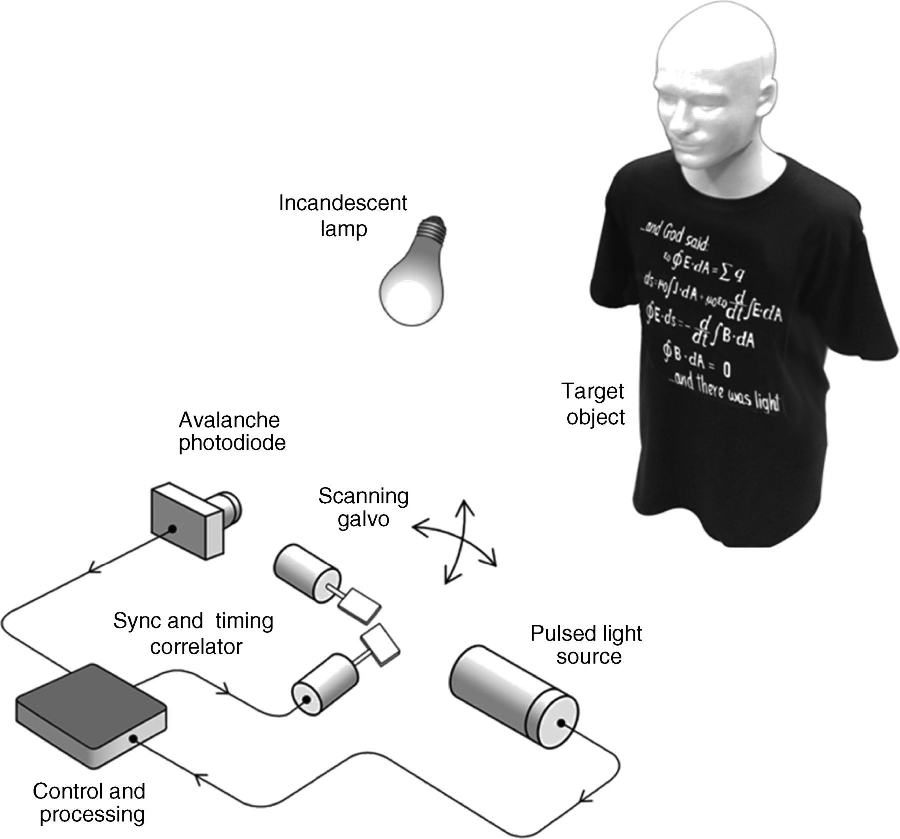
\includegraphics[width=14cm]{figure-first-setup.pdf}}
\caption{Schematic of the raster-scanning imager used for first-photon imaging.}
\label{figure:first-setup}
\end{figure}

A diagram of our raster-scanning active imager is shown in Figure \ref{figure:first-setup}. The illumination source was a PicoQuant LDH series pulsed laser diode with a center wavelength of 640 nm, a tunable repetition rate of 5 - 80 MHz that was set at 10 MHz for this experiment. As with most pulsed laser diode sources, the pulse shape and duration is dependent on the power, so we fixed our average power setting at 0.6 mW, which gave us pulses with 226 ps RMS duration, as shown in Figure \ref{figure:first-pulse}.

The laser output was reflected off a Thorlabs GVS012 two-axis scanning galvo system that raster scanned the beam over the target. The maximum mechanical scan angle was $\pm 20^\circ$, which was the limit on our field of view. The galvo system took two analog voltage inputs (one for each axis, 0.5 V/deg) which we supplied using a National Instruments NI USB-6008 module that contained two 12-Bit analog outputs with a maximum sample rate of 1 kHz.

We placed our objects at distances of 1.5 to 2 m from the illumination source. The diameter of the spot size at 2 m distance was measured to be $\sim$1.5 mm. Prior to detection, the light was filtered using an Andover custom free-space interference filter with 2 nm bandwidth centered at 640 nm whose peak transmission was 49\%. The Geiger-mode APD was a Micro Photon Devices PDM series detector with 100 $\mu$m $\times$ 100 $\mu$m active area, 35\% quantum efficiency, less than 50 ps timing jitter, and less than $2\times 10^4$ dark counts per second. The photon detection events were time stamped relative to the laser pulse with 8 ps resolution using a PicoQuant HydraHarp TCSPC module. The laser and the single-photon detector were placed in the same horizontal plane, at a separation of 7 cm, making our imaging setup effectively monostatic.

Prior to measurement, a HydraHarp time-tagged time-resolved (T3) measurement was initiated remotely over a network connection. We performed the raster scan using a custom Visual C\# program that includes correction for the perspective distortion caused by the mounting of the galvo mirror. In addition, the custom program applies a specific pattern to reverse the raster scanning direction, as shown in Figure \ref{figure:first-scanning}, the custom program employed smooth scanning that avoided abrupt mechanical transitions between rows. Before each movement of the galvo mirror position, a pixel marker pulse was simultaneously output to a designated digital output of a USB-6008 that was connected to a Stanford Research Systems delay generator. The delay generator then produced a pulse compatible with the HydraHarp marker input in order to insert a marker into the data stream indicating a pixel position change. A final marker signal was output after the last pixel as well, accounting for a total of $N^2+1$ markers in each file for an $N \times N$-pixel image. The resulting HT3 files are read using a custom GNU C program (see Appendix \ref{appendix:ht3read}) based on PicoQuant file specifications. This program discards the data prior to the first pixel and after the end of the measurement, and outputs a MATLAB-friendly ASCII file describing all the marker and photon detection events. For photon detection events, the C program additionally outputs the laser pulse number and the time bin in which the detection was received. For marker events, the C program outputs the total number of photons detected since the last marker and the sum of the time bin values since the last marker, allowing for convenient retrieval of the traditional averaging (ground truth) measurement. The C program also has an option to only output the first few photon detections after each marker, to reduce data storage as converting the entire .ht3 file to ASCII format would occupy several tens of gigabytes. The output ASCII format is illustrated in Figure \ref{figure:first-outformat}.

\begin{figure}[htb]
\centerline{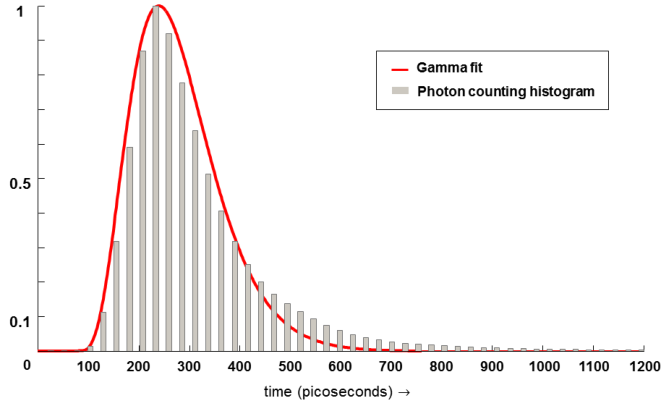
\includegraphics[width=14cm]{figure-first-pulse.pdf}}
\caption{Pulse shape of the PicoQuant LDH series laser diode obtained by histogramming, and skewed Gamma function fit.}
\label{figure:first-pulse}
\end{figure}

\begin{figure}[htb]
\centerline{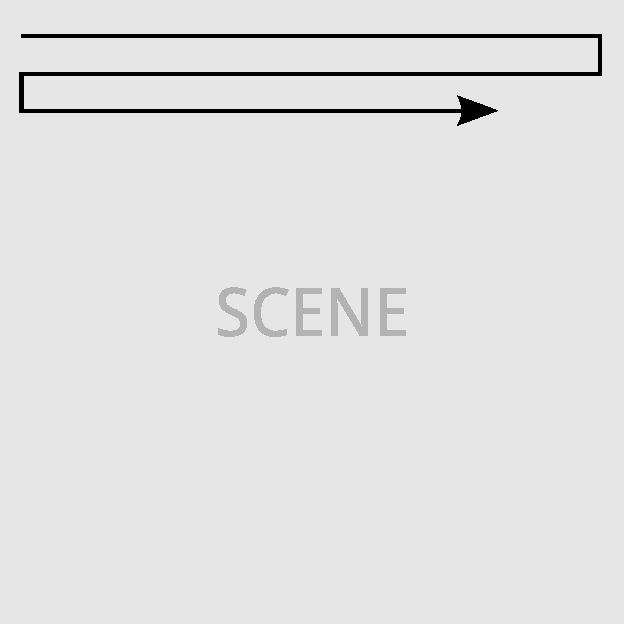
\includegraphics[width=9cm]{figure-first-scanning.pdf}}
\caption{Raster scanning was performed in alternating directions for each row in order to avoid abrupt transitions in translating the galvo mirrors.}
\label{figure:first-scanning}
\end{figure}

\begin{figure}[htb]
\centerline{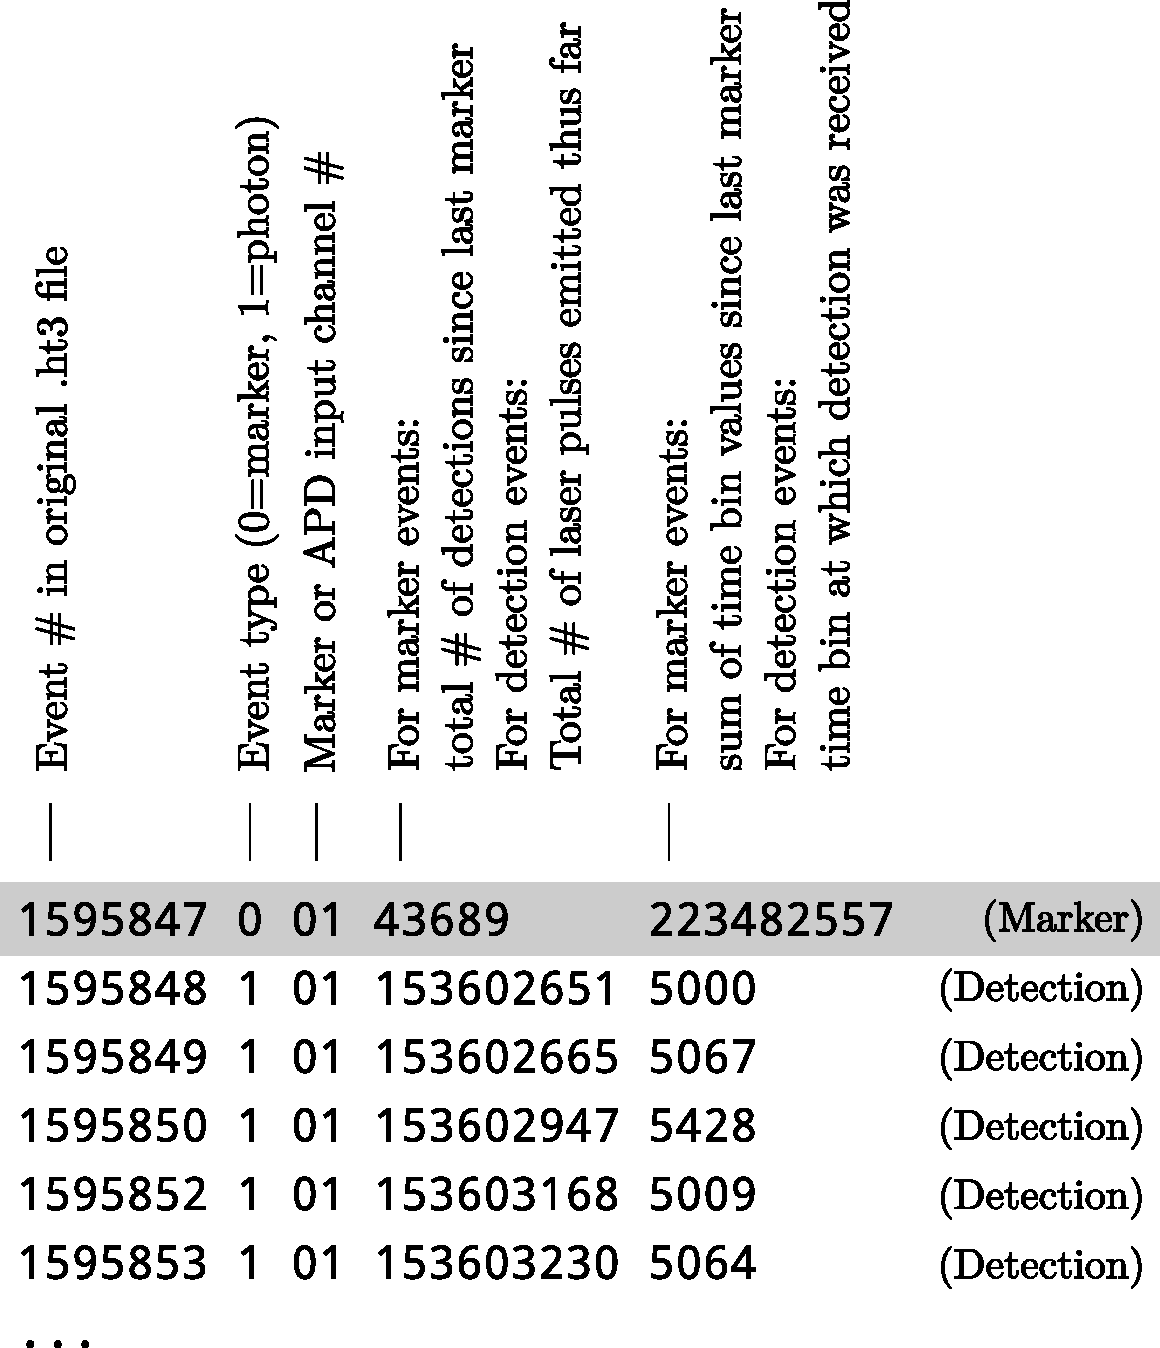
\includegraphics[width=10cm]{figure-first-outformat.pdf}}
\caption{Description of the MATLAB-friendly .out format generated by our custom GNU C .ht3 file reader.}
\label{figure:first-outformat}
\end{figure}

\subsubsection{Focusing of laser beam}
As with most diode lasers, the output of the PicoQuant LDH series laser diode is multimodal and not very well collimated beyond a range of several tens of centimeters. Since a large spot size would reduce our transverse resolution, we mitigated this problem by using a pair of 12-cm focal length lenses to loosely focus the beam such that the spot size was small ($\sim$1 mm) over the 1.5-m to 2-m range where we placed the object.

\subsubsection{Addition of background noise}
In order to simulate a realistic imaging scenario with background light, we placed an incandescent lamp in the room pointed at the detector, and set the background light level to roughly match the signal level (i.e. the probability of any detection being due to background light would be around 50\%). We set this level by first turning off the incandescent source and using the laser to illuminate a reference point on a highly-reflective Lambertian surface at a distance of 2 m, measuring the average detected photon rate, and then matching that rate by adjusting the current input to the incandescent source.

\subsubsection{Photon flux waveform measurement}
For range estimation, our computational imager requires knowledge of the photon-flux waveform of the laser pulses. We use $s(t)$ to denote the normalized ($\int s(t) dt = 1$) version of this
waveform for a laser pulse emitted at $t = 0$. This pulse shape was measured by directly
illuminating the detector with highly attenuated laser pulses and binning the photon arrival times
to generate a histogram of photon counts. Fitting a skewed Gamma function to this histogram
yields:
\begin{equation}
s(t) = A (t - T_s)^4 \exp \left( -\frac{t-T_s}{T_c} \right)
\end{equation}
where $T_s$ = 80 ps, $T_c$ = 40 ps, and $A>0$ is the normalization constant, as shown in Figure \ref{figure:first-pulse}.

\subsubsection{Acquisition procedure}
To generate one complete data set, we raster scanned over 1000 $\times$ 1000 pixels with the two-
axis galvo. At transverse pixel location $(x, y)$, we implemented a first-photon imager that records only two values: $n(x, y)$, the number of laser pulses transmitted prior to the first detection event; and $t(x, y)$, the timing of the detection relative to the pulse that immediately preceded it. An ideal first-photon imager would move to the next pixel immediately after a single detection event.
In our case, it is not possible to build such a fast scanner, because we are physically limited by the mechanical speed of our galvo mirror system; at the fastest scanning rate we typically observe tens or even hundreds of photon arrivals at each pixel. Faster scanning may be achievable using smaller galvo mirrors or digital micromirror arrays. We are also limited by the 1 kHz sampling rate of our digital-to-analog converter, which permits a fastest acquisition of a little under 17 minutes for a 1-megapixel image. Without these physical raster scanning limitations, our photon flux is high enough for much faster acquisition.

In order to compare our first-photon imaging method with traditional acquisition techniques, we need to perform a baseline measurement with traditional histogramming. In order to do this we deliberately slowed down the acquisition to approximately 3 hours per image in order to collect enough photon arrivals at each pixel to obtain a clean histogram of a few thousand arrivals at each pixel. Our reference images are constructed from averaging over $\sim$1000 arrivals at each pixel, and are generated only for comparison purposes. For our novel first photon imaging method, we only utilized the first arrival at each pixel and discarded all subsequent data.

Because our entire scene was contained within a few meters of the imaging setup, our 100 ns pulse repetition period guaranteed that each non-background photon detection came from the immediately preceding laser pulse.

\begin{figure}[htb]
\centerline{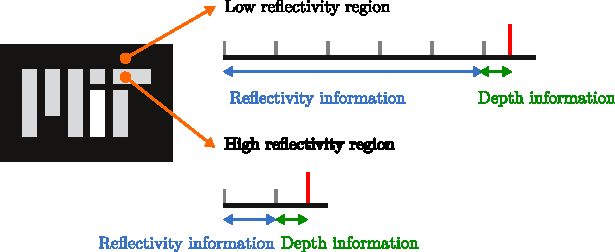
\includegraphics[width=14cm]{figure-first-pulses.pdf}}
\caption{Reflectivity and depth information obtained from a single photon arrival: the depth information is obtained by measuring the time difference between the photon arrival and the laser pulse sync signal, while the reflectivity information is obtained by the number of laser pulse periods elapsed until the first photon detection.}
\label{figure:first-pulses}
\end{figure}

\subsection{Computational reconstruction procedure}

In this section we present a 3-step computational reconstruction procedure that we used to recover high quality scene reflectivity and depth data from the first photon arrival data. A. Kirmani, D. Shin, A. Colaco, V. Goyal, and J. Shapiro developed the theoretical framework outlined below \cite{kirmani-first,kirmani-photon} with feedback from early experimental data.

\subsubsection{Reflectivity reconstruction}

Traditional imaging techniques typically count photon arrivals to measure reflectivity. However, given only a single arrival, the only information we obtain about reflectivity is the time duration (i.e., number of laser pulse repetition periods) until a photon is detected, as shown in Figure \ref{figure:first-pulses}. Since brighter regions reflect a greater number of photons, the mean time duration until a photon is detected is shorter. This is characterized by Poisson statistics. Let $S$ be the average photon number in the back-reflected signal from a hypothetical unity-reflectivity spatial location illuminated by the laser pulse, $\alpha(x,y)$ denote the scene reflectivity at pixel location $(x,y)$, $B$ denote the background photon arrival rate, $T_r$ be the pulse repetition period, and $\gamma$ be the efficiency of the detector. The probability of not detecting a photon is then
\begin{equation}
P_0(x, y) = \exp\left(-\gamma[\alpha(x,y)S + BT_r]\right)\,\,.
\label{equation:first-probdetect}
\end{equation}
Since these probabilities are independent and identically distributed (iid) for each pulse, it follows that the number of pulses until a detection, denoted by $n(x, y)$, is geometrically distributed:
\begin{equation}
\operatorname{Pr}\left[n(x,y) = k \right] = P_0(x,y)^{k-1} \left[ 1 - P_0(x,y) \right]\,\,.
\label{equation:first-geometric}
\end{equation}

When there is no background light present, the maximum likelihood (ML) estimate of the reflectivity at each pixel $\hat{\alpha}_{ML}(x,y)$ is proportional to $1/n(x,y)$ for $n(x,y) \gg 1$. In the presence of high background light ($B T_r \gg \alpha(x,y) S$) this estimate becomes severely corrupted since it is much more likely that a background photon will reach the detector before a signal photon.

In order to perform a sparsity-promoting computational reconstruction of the reflectivity from this data, we first compute the negative log-likelihood of the ML estimate using Eqs. \ref{equation:first-probdetect} and \ref{equation:first-geometric}, which is shown to be \cite{kirmani-first}:
\begin{equation}
\mathcal{L}\left( \alpha(x,y) | n(x,y) \right) = \gamma \left[ \alpha(x,y) S + B T_r \right] \left[ n(x,y) - 1 \right] - \log \left\{ \gamma \left[ \alpha(x,y) S + B T_r \right] \right\}\,\,,
\end{equation}
where $\gamma\left[\alpha(x,y)S + BT_r\right] \ll 1$ has been assumed.
We must also choose a sparsity-promoting basis for reconstruction. Most objects are characterized by smoothly-varying surfaces punctuated by sharp edge transitions; this type of sparsity is captured well by most wavelet bases which are localized in both space and frequency. Bases such as the Fourier Transform or Discrete Cosine Transform, which only localize frequency and not space, require a large number of nonzero basis elements to describe sharp edges and are not typically the best choice for these types of objects, but may be a more suitable choice for imaging scenes that do not contain edges. In our case we used the discrete wavelet transform (DWT) derived from Debauchie's 4-tap filters \cite{mallat-wavelet}. Using $\Phi\left(\cdot\right)$ to denote the wavelet transform, which is implemented in the form of matrix multiplication, the wavelet coefficients are $\left\{ w(x,y) \right\} = \Phi(\left\{ \alpha(x,y) \right\})$ for the collection of reflectivity estimates $\left\{ \alpha(x,y) \right\}$ for all pixel coordinates $(x,y)$. A standard measure of sparsity, similar to that which we used in compressed sensing in the previous chapter, is the $\ell_1$-norm of these coefficients, defined by:
\begin{equation}
|| \Phi\left(\left\{ \alpha(x,y) \right\}\right) ||_1 = \sum_x \sum_y | w(x,y) |\,\,.
\end{equation}

We would like to reconstruct the reflectivity estimate by minimizing a weighted sum of both the negative log-likelihood and the sparsity measuring function over the set of all possible images $\left\{\alpha(x,y)\right\}$. This prevents the estimate from deviating too far (quantified by the probability distribution itself) from the measured data, while regularizing it to be as spatially sparse as possible (quantified by the chosen DWT basis). The optimization program can be written as the minimization of
\begin{equation}
\{ \hat{\alpha}(x,y) \} = \underset{\{\alpha(x,y)\}}{\operatorname{arg\,min}} \left\{ (1 - \beta) \left[ \sum_x \sum_y \mathcal{L}( \alpha(x,y) | n(x,y) ) \right] + \beta || \Phi\left(\left\{ \alpha(x,y) \right\}\right) ||_1 \right\}
\label{equation:alpha-est}
\end{equation}
subject to $\hat{\alpha}(x,y) \geq 0$ for all $(x,y)$. Since the negative log-likelihood function is convex in $\alpha(x,y)$, and the sparsity-promoting function is also convex \cite{boyd-convex}, so too is their nonnegative weighted sum. Convexity enables us to efficiently find the global minimum solution to $\left\{ \alpha(x,y) \right\}$ by iteratively searching for a local minimum.

The two terms of the optimization program in Eq. \ref{equation:alpha-est} can be thought of as penalty factors; the first penalizes results that are too far from the measured data, and the second penalizes results that are not spatially sparse in the wavelet basis. The parameter $\beta$, where $0 < \beta < 1$, determines the weighting between these two penalty factors; each choice of $\beta$ produces a candidate reflectivity image. We choose $\beta$ by scanning from 0.1 to 0.9 in steps of 0.1 and selecting the value that minimizes the objective function in Eq. \ref{equation:alpha-est} \cite{kirmani-first}.

\subsubsection{Background noise censoring}

Before reconstructing the depth map of our object, we wish to eliminate the photon arrivals that are due to the background light and provide no information about depth. We do this by taking advantage of the fact that anomalous detections due to background light are independently and uniformly distributed over $[0, T_r]$ with a high variance of $T_r^2/12$ (following from the uniform probability distribution), whereas detections from back-reflected signal pulses are temporally concentrated and spatially correlated with signal detections from nearby pixels.

We approach the censoring of noise photons by computing the rank-ordered absolute differences (ROAD) statistic \cite{garnett-universal} for each pixel. For each pixel, we use the photon arrival times of its eight nearest neighbors and then perform a binary hypothesis test to decide whether the photon is due to background or noise with high probability. This binary hypothesis test is dependent on the reflectivity of the object at that pixel, which we recovered in the previous step (this is the reason why noise censoring cannot be done prior to reflectivity reconstruction, although it may be possible to consider an iterative procedure). We then delete the anomalous arrival-time values before performing depth reconstruction.

The ROAD statistic is calculated as follows: for each pixel $(x,y)$, we take the eight neighboring pixels $(x_1,y_1) ... (x_8,y_8)$ and compute the time-of-arrival differences with the current pixel:
\begin{equation}
|t(x_1,y_1) - t(x,y)| , \, ... \, , |t(x_8,y_8) - t(x,y)|
\end{equation}
We then sort these values in ascending order, and define $\operatorname{ROAD}(x,y)$ to be the sum of the first four values in the sorted list.

We then use a binary hypothesis test to classify whether the photon arrival at $(x,y)$ is due to signal light or background light. We combine our knowledge of the reflectivity estimate $\hat{\alpha}(x,y)$ which we obtained in the previous step with theory of merged Poisson processes \cite{bertsekas-introduction} to obtain the probabilities:
\begin{equation}
\operatorname{Pr}[\mathrm{background}] = \frac{BT_r}{\hat{\alpha}(x,y)S + BT_r}
\end{equation}
\begin{equation}
\operatorname{Pr}[\mathrm{signal}] = 1 - \frac{BT_r}{\hat{\alpha}(x,y)S + BT_r}
\end{equation}

We then generate the threshold $C$ used for a binary hypothesis test as follows:
\begin{equation}
C = 4T_p \frac{ BT_r }{\hat{\alpha}(x,y)S + BT_r}
\end{equation}
where if $\operatorname{ROAD}(x,y) \geq C$, we decide that the photon arrival is due to background lightand delete that data, and if $\operatorname{ROAD}(x,y) < C$, we keep the data point. This method works with high reliability \cite{garnett-universal} as long as the variance of signal photon arrival times is much smaller than the variance of the uniform distribution of background photon arrivals.

\subsubsection{Depth reconstruction}
The approach to reconstruction of the depth map of the object is similar to that of the reflectivity reconstruction approach. For each pixel $(x,y)$ we first compute the negative log-likelihood function relating the signal photon's arrival time $t(x,y)$ to the depth map of the scene $Z(x,y)$ in distance units. This is given by:
\begin{equation}
\mathcal{L}(Z(x,y) | t(x,y)) = -\log\left[ s(t(x,y) - \frac{2Z(x,y)}{c}) \right]
\label{equation:depth-ll}
\end{equation}
where $s(\cdot)$ is the pulse shape given earlier, $c$ is the speed of light, and the factor of 2 is incurred due to the round-trip distance from the emitter to the object and back to the detector. Equation \ref{equation:depth-ll} assumes that $\gamma[\alpha(x,y)S + BT_r] \ll 1$ and that background light censornig has been effective \cite{kirmani-first}. We insert the fitted $s(\cdot)$ we determined earlier to obtain:
\begin{equation}
\mathcal{L}(Z(x,y) | t(x,y)) = -4\log\left[ t(x,y) - \frac{2Z(x,y)}{c} \right] - \frac{t(x,y) - T_s - 2Z(x,y)/c}{T_c}\,\,.
\end{equation}
This negative log-likelihood function is strictly convex in $Z(x,y)$, which we again require for efficient computational reconstruction.

Similar to the reflectivity construction program in Eq. \ref{equation:alpha-est}, we measure sparsity using the $\ell_1$-norm of the wavelet transform of $Z(x,y)$ and form a reconstruction of the depth image by solving
\begin{equation}
\{ \hat{Z}(x,y) \} = \underset{\{Z(x,y)\}}{\operatorname{arg\,min}} \left\{ (1 - \beta) \left[ \sum_x \sum_y \mathcal{L}( Z(x,y) | t(x,y) ) \right] + \beta || \Phi\left(\left\{ Z(x,y) \right\}\right) ||_1 \right\}
\label{equation:depth-est}
\end{equation}
subject to $\hat{Z}(x,y) \geq 0$ for all $(x,y)$. Also similar to Eq. \ref{equation:alpha-est}, $\beta$ is a weighting parameter between the two penalty factors and is chosen by scanning from 0.1 to 0.9 and choosing the value that minimizes the objective function. Note that in Eq. \ref{equation:depth-est}, the summation only includes the uncensored data points.

\subsubsection{Software implementation}
We employed the SPIRAL-TAP package for MATLAB \cite{harmany-spiral} to implement the optimization programs described for the reflectivity and depth reconstructions. The background noise censoring is implemented directly in MATLAB. To initialize the convex optimizer in reflectivity reconstruction, we use the pointwise ML estimate:
\begin{equation}
\alpha_{ML}(x,y) = \operatorname{max}\left\{ \frac{1}{\gamma S (n(x,y) - 1)} - \frac{BT_r}{S}, 0 \right\}\,\,.
\end{equation}

To initialize the depth estimator, we used the ML estimate
\begin{equation}
Z_{ML}(x,y) = (t(x,y) - T_m)c/2
\end{equation}
where $T_m = \operatorname{arg\,max} s(t)$ where $(x,y)$ has an uncensored arrival time, and $Z(x,y) = 0$ where $(x,y)$ has a censored arrival time. Full code and sample data are available as supplementary materials online \cite{kirmani-first}.

\subsection{Results}

\subsubsection{Mannequin}
Our main imaging target was a life-size plastic mannequin wearing a black T-shirt with white text. We chose this not only as an example of a realistic target, but also as one which has both depth and intensity features on multiple scales.

Figure \ref{figure:first-manflower} shows separate reflectivity and depth images of an early measurement scanned at a lower resolution of 300$\times$300 that was obtained with the mannequin placed next to a sunflower and without background light injection. This figure includes reference (ground truth) measurements, point-wise ML estimates from a first-photon acquisition, and the result of our computational reconstruction. We see that our algorithm is able to recover fine features, particularly the petals of the flower and facial features of the mannequin seen in the reference image, that are absent from the point-wise ML estimates.

We then switched on the incandescent lamp to the level described earlier and found our reconstruction method to perform surprisingly well under such high background levels. Figure \ref{figure:first-mannequin} shows the results of this measurement, displayed as reflectivity superimposed on a 3D scatter plot of the depth data from raw data to each step of data processing described above; all pictures are generated from the same data set consisting of one photon detection per pixel. We notice that the reflectivity reconstruction is able to recover sufficient detail to resolve fine text on the T-shirt, a close-up of which is shown in Figure \ref{figure:first-mannequin-zoom}. Background noise censoring and depth reconstruction are also able to recover many facial feature details that are almost impossible to make out in the raw data.

\begin{figure}[h!]
\centerline{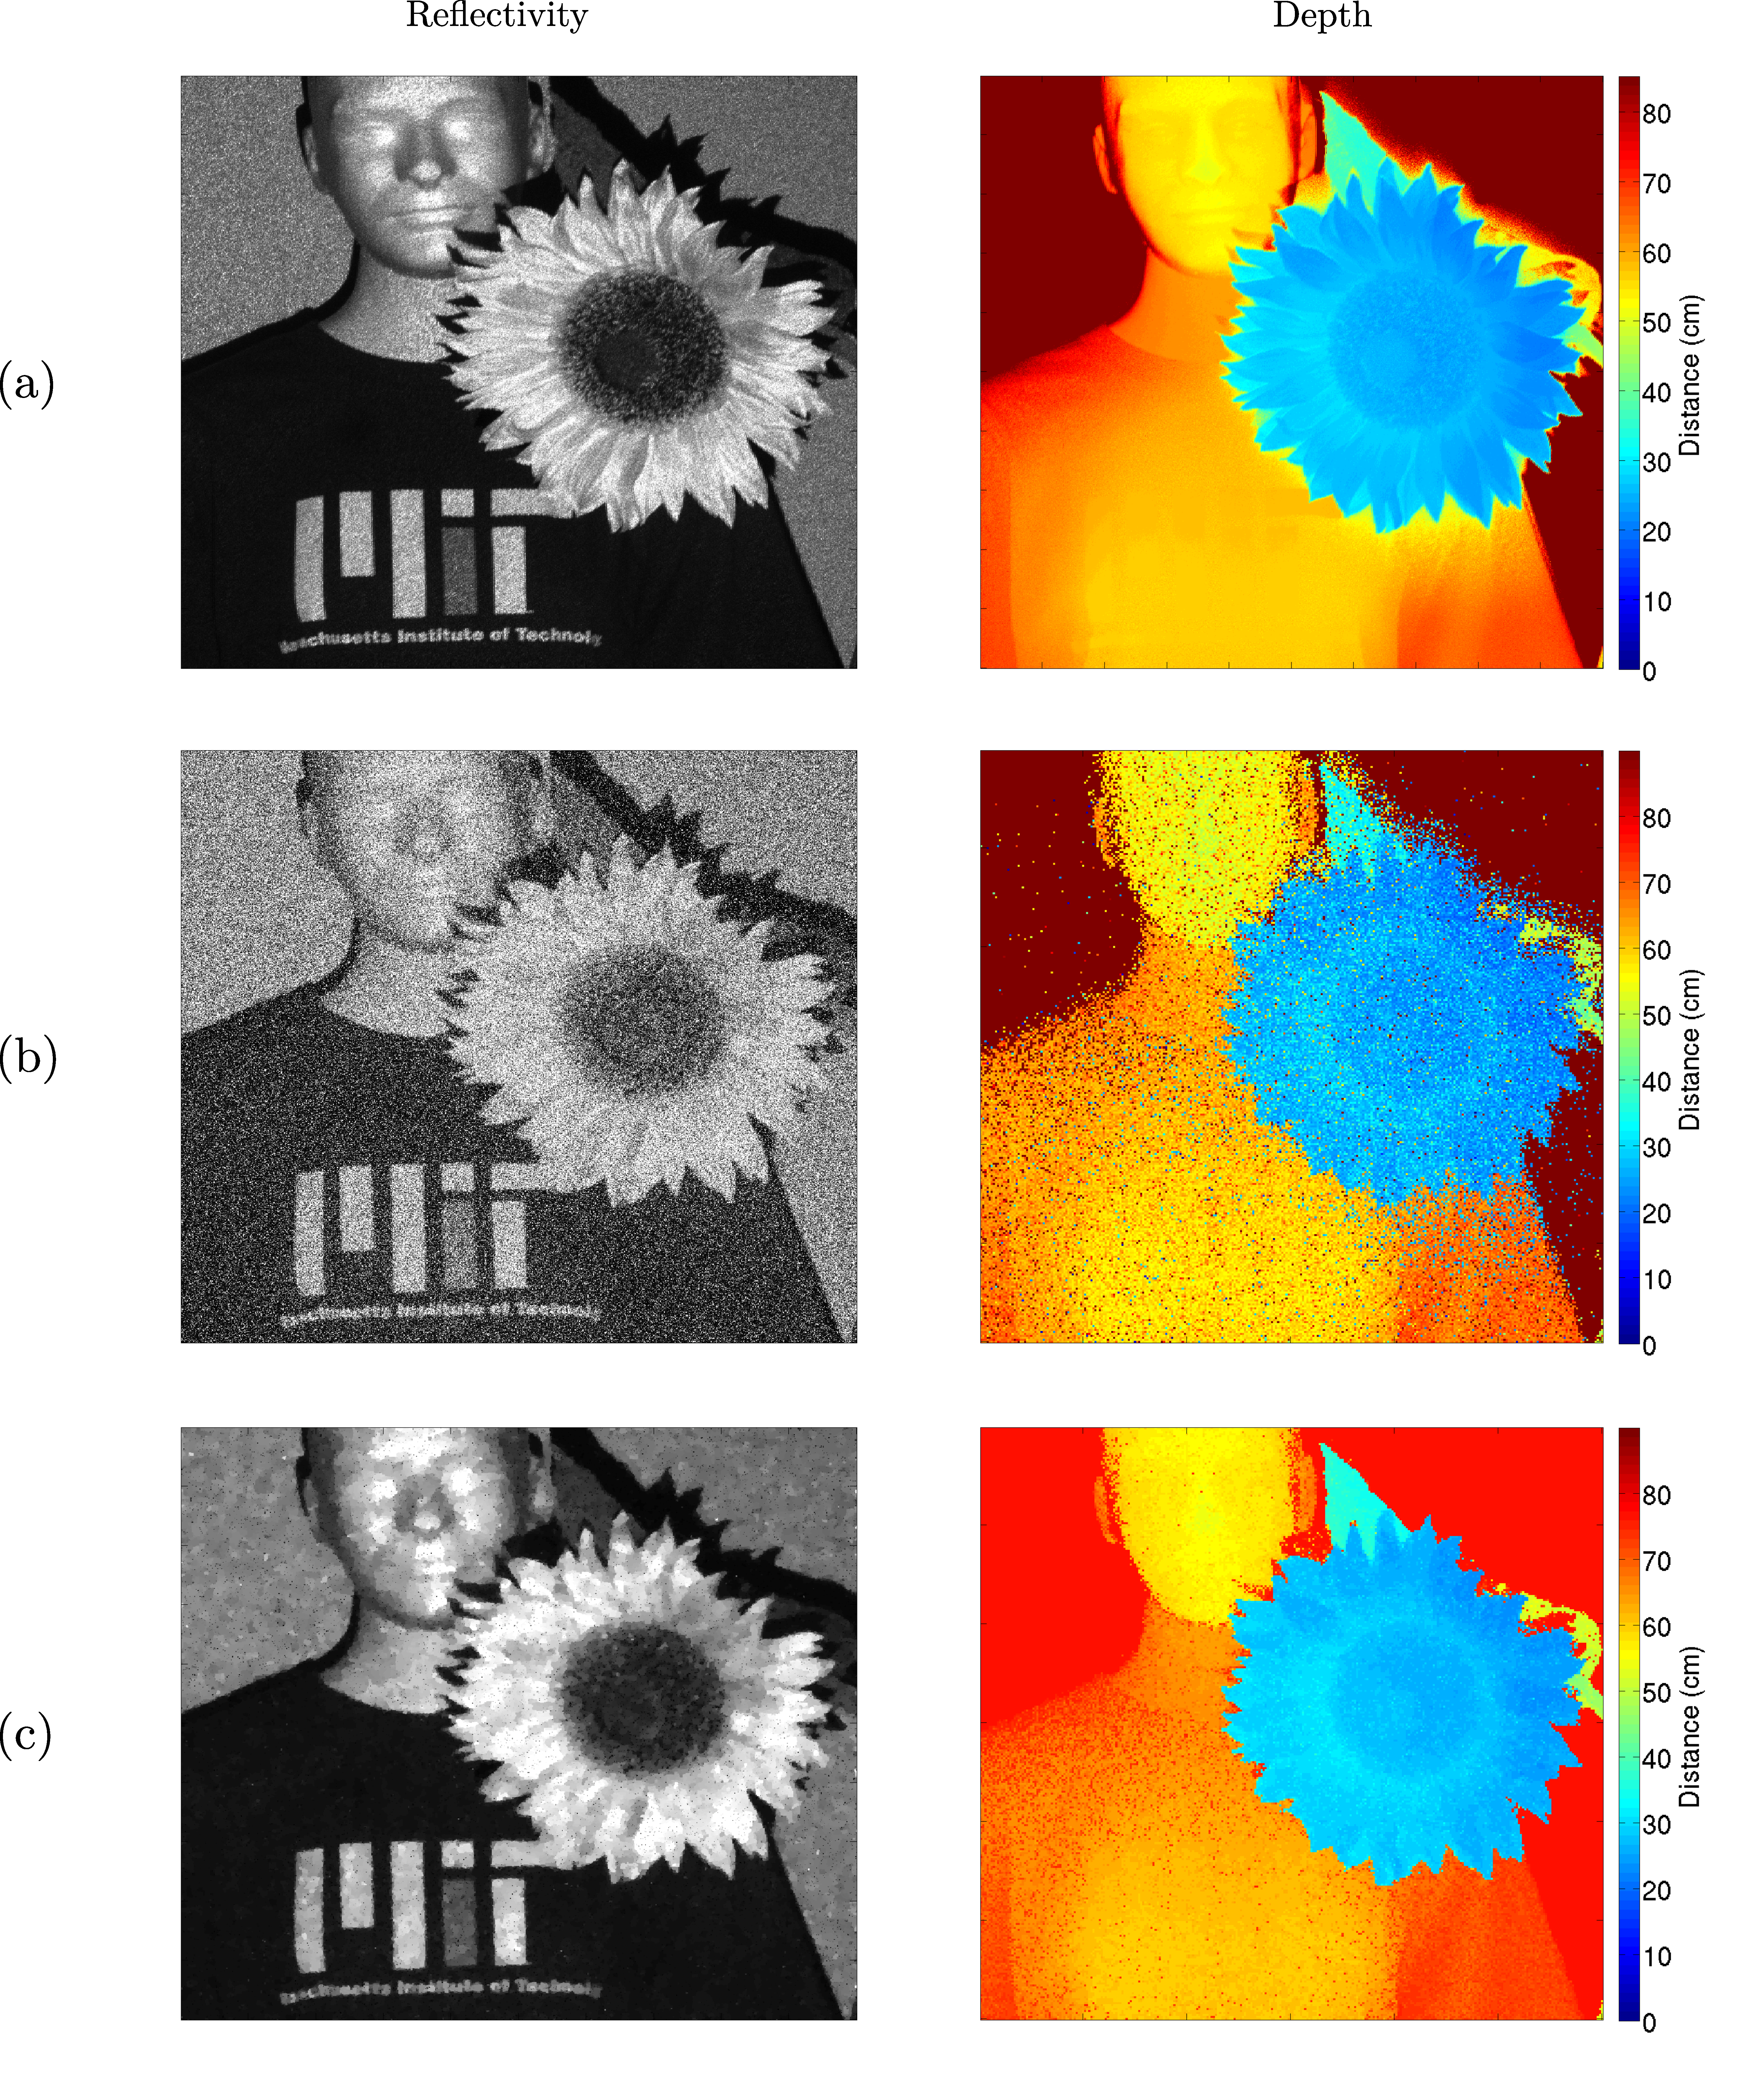
\includegraphics[width=0.9\textwidth]{figure-first-manflower.pdf}}
\caption{Early reflectivity and depth images of a mannequin and flower scene imaged using a 300$\times$300-pixel raster scan without background light injection. (a) Reference (ground truth) measurement obtained by averaging several hundred photon arrivals at each pixel. (b) Pixel-wise ML estimates obtained using only the first photon arrival at each pixel. (c) Our computational reconstruction method applied to the data in (b).}
\label{figure:first-manflower}
\end{figure}

\begin{figure}[h!]
\centering
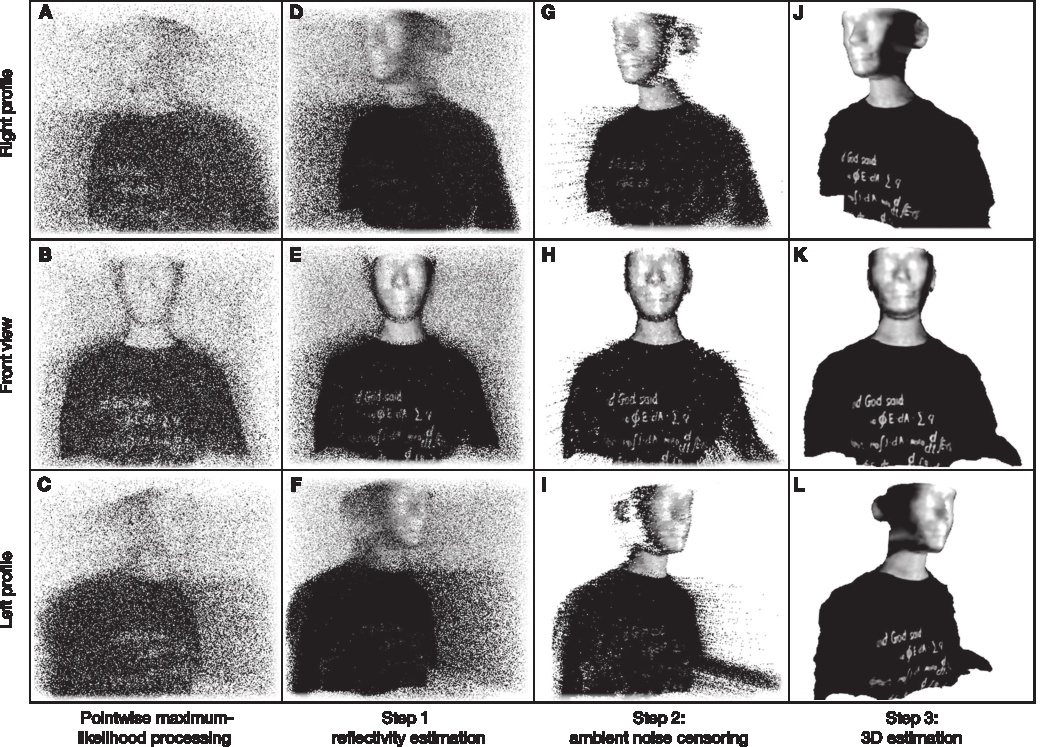
\includegraphics[width=\textwidth]{figure-first-mannequin.pdf}
\caption{3D mesh views of a single first-photon acquisition with added background noise after various stages of processing. (A)-(C): Raw reflectivity ML estimate $\alpha_{ML}(x,y)$ superimposed over depth ML estimate $Z_{ML}(x,y)$ from first photon data, (D)-(F): after reflectivity reconstruction of $\alpha(x,y)$, (G)-(I): after background noise censoring, (J)-(L): after depth reconstruction of $Z(x,y)$.}
\label{figure:first-mannequin}
\end{figure}


\begin{figure}[h!]
\centerline{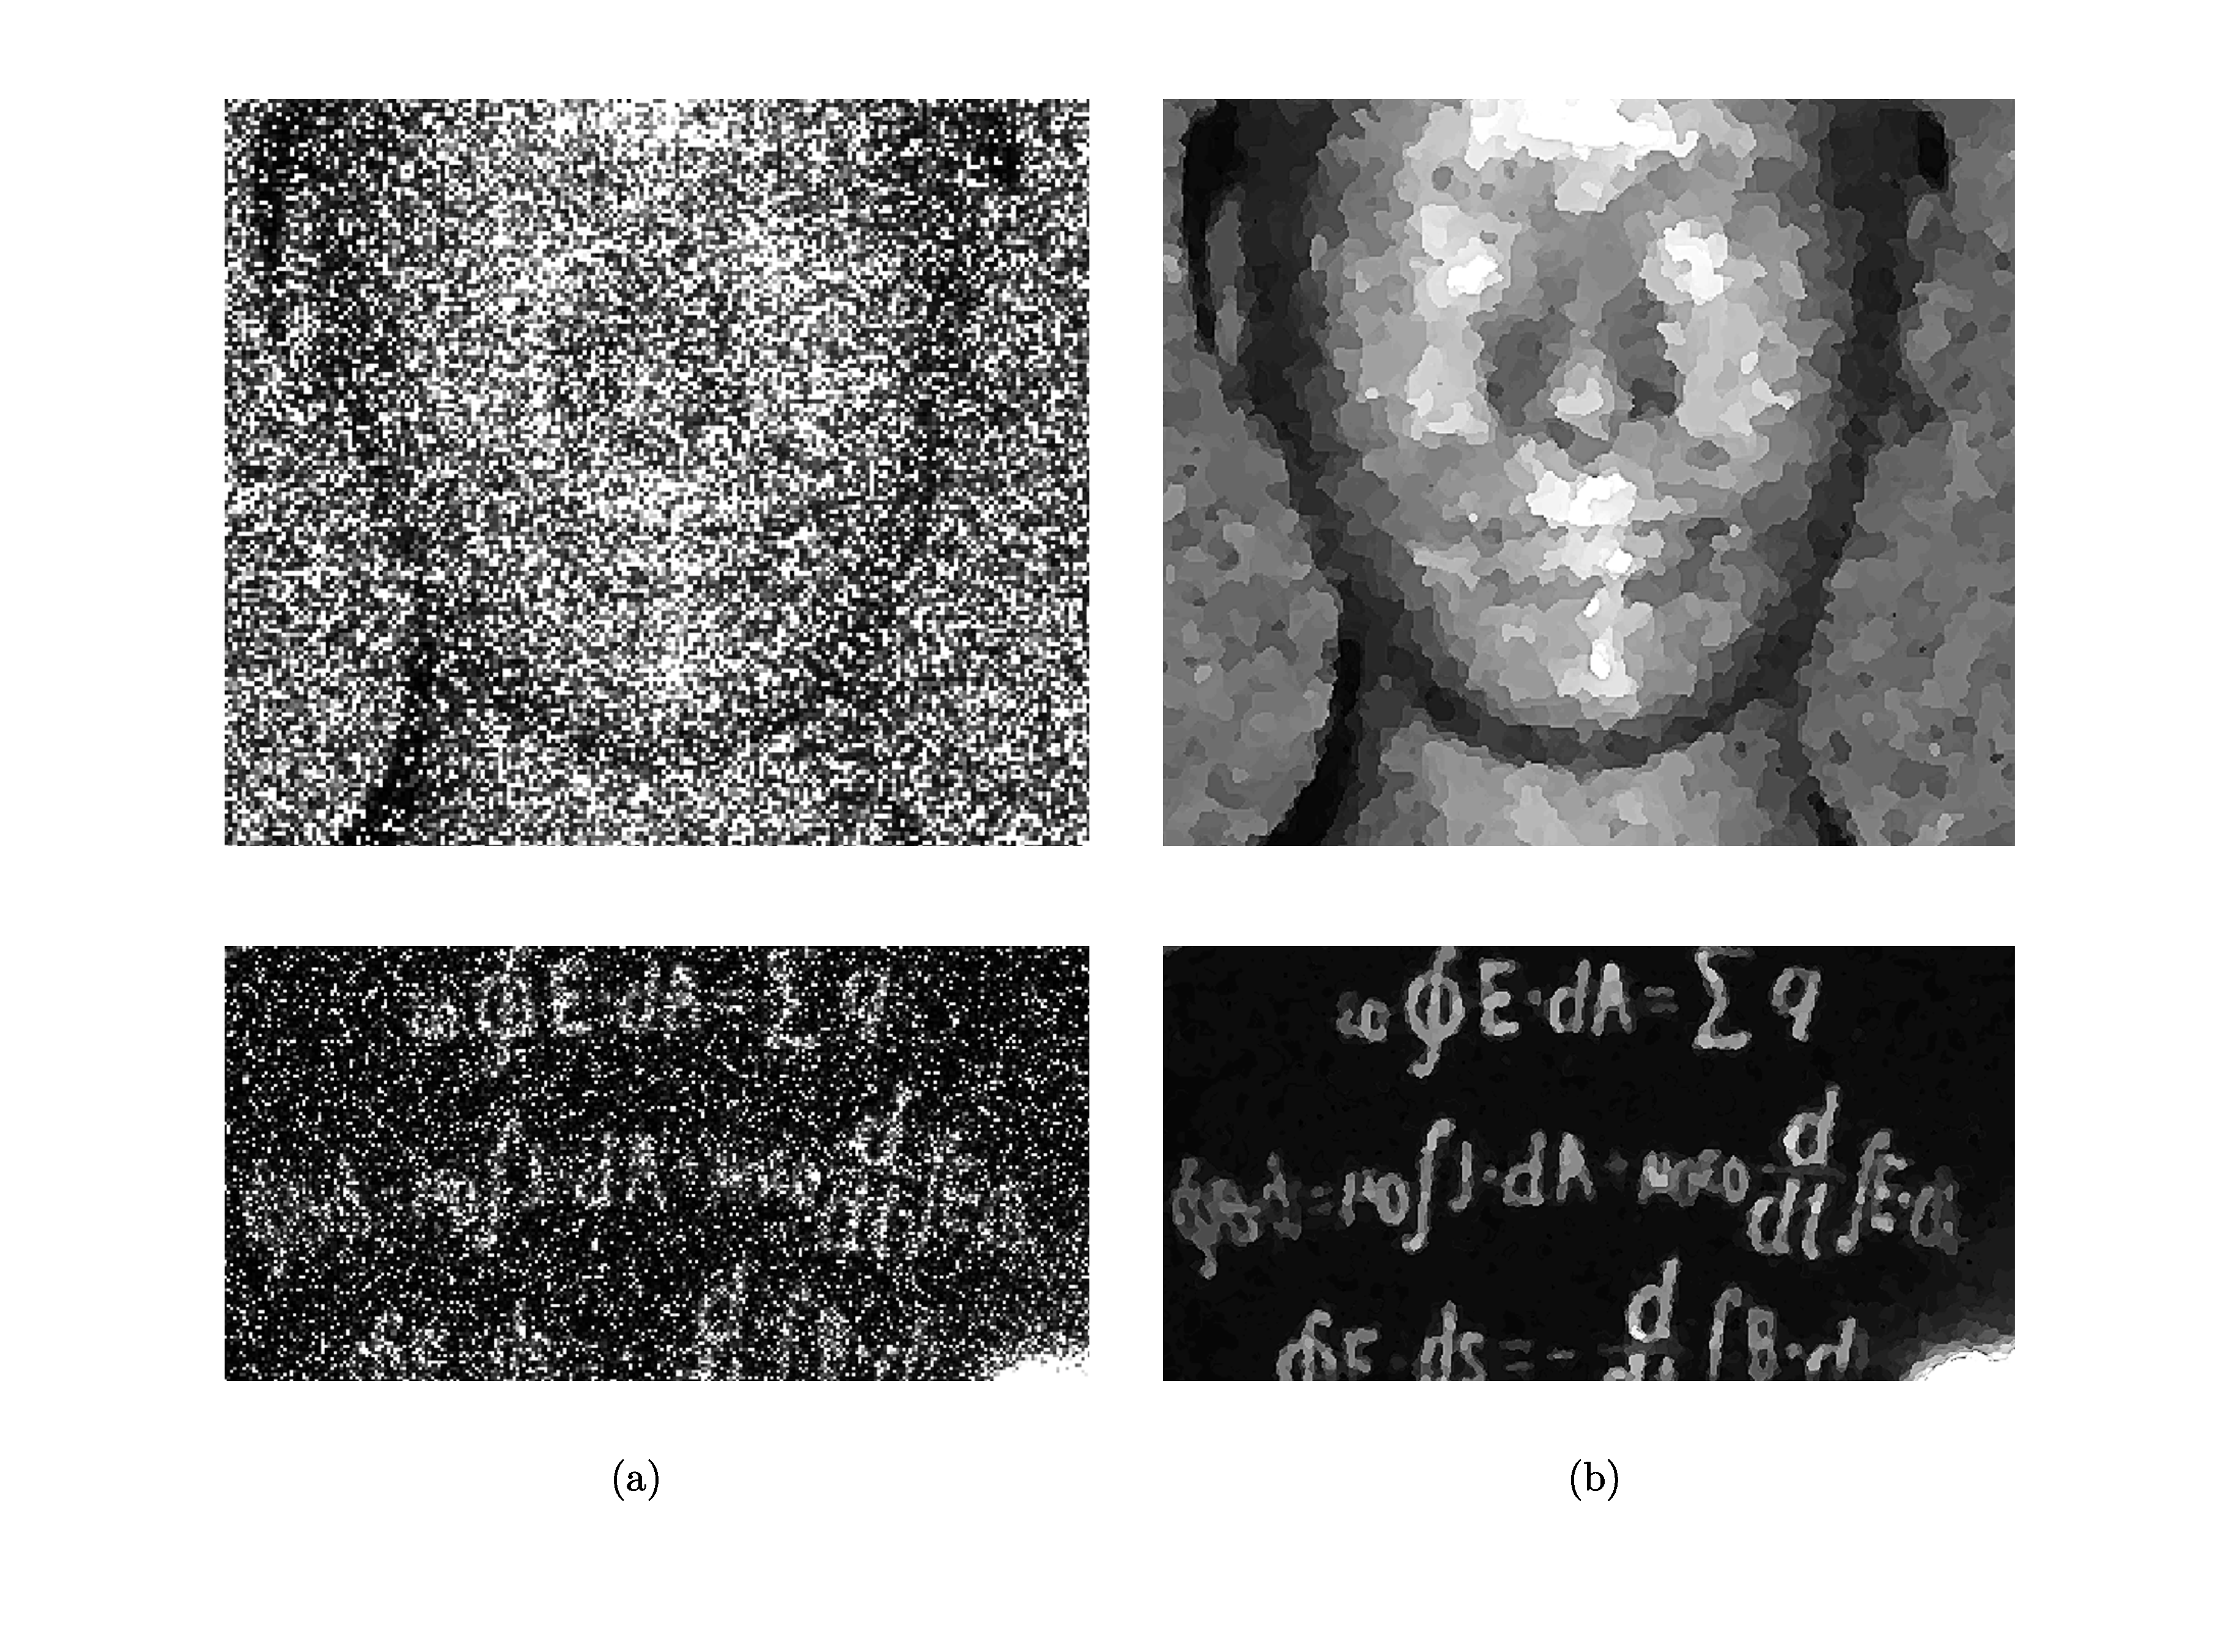
\includegraphics[width=\textwidth]{figure-first-mannequin-zoom.pdf}}
\caption{Close-up of two regions of reflectivity data for mannequin target. (a) Pixel-wise ML estimate using only 1 photon per pixel and (b) the same data after processing using our computational reconstruction technique.}
\label{figure:first-mannequin-zoom}
\end{figure}

\subsubsection{Depth chart}

To independently analyze the depth-resolving capabilities of our computational reconstruction technique, we constructed and imaged a depth chart consisting of a flat board with 5$\times$5 embossed rectangular plastic squares, as shown in Figure \ref{figure:first-depthchart}. Each square had transverse dimensions of 5$\times$5 cm and the axial heights linearly increased in steps of $\sim$3.2 mm along both axes. The entire board was spray-painted using a single color of matte-finish paint for near-constant Lambertian reflectivity. We first took a reference (ground truth) measurement by accumulating and averaging hundreds of arrivals at each pixel, as shown in Figure \ref{figure:first-depthchart}(a), which clearly shows all 25 squares. Although the board itself was flat, the depth images incurred spherical distortion due to angular raster scanning.

Figure \ref{figure:first-depthchart}(b) shows the pixel-wise ML estimate of the depth taken only from the first photon arrival at each pixel. Since our axial feature size was on the order of $\sim$3.2 mm and our RMS pulse duration was $\sim$226 ps which multiplied by the speed of light corresponds to 67 mm, it is natural to expect that objects significantly smaller than the pulse width would be almost impossible to resolve without averaging; this is indeed the case with the pixel-wise ML estimate. However, as we see in Figure \ref{figure:first-depthchart}(c), the same data processed through our computational reconstruction technique resolved depth features as small as 6.4 mm, demonstrating a factor-of-10 sub-pulse depth resolution improvement. This is explained by the fact that the ML estimates do not take into account spatial regularity, whereas our computational reconstruction approach promotes smooth surfaces with few sharp transitions, making use of data from several pixels at once to extract these features that are otherwise almost invisible.

\begin{figure}[h!]
\centering
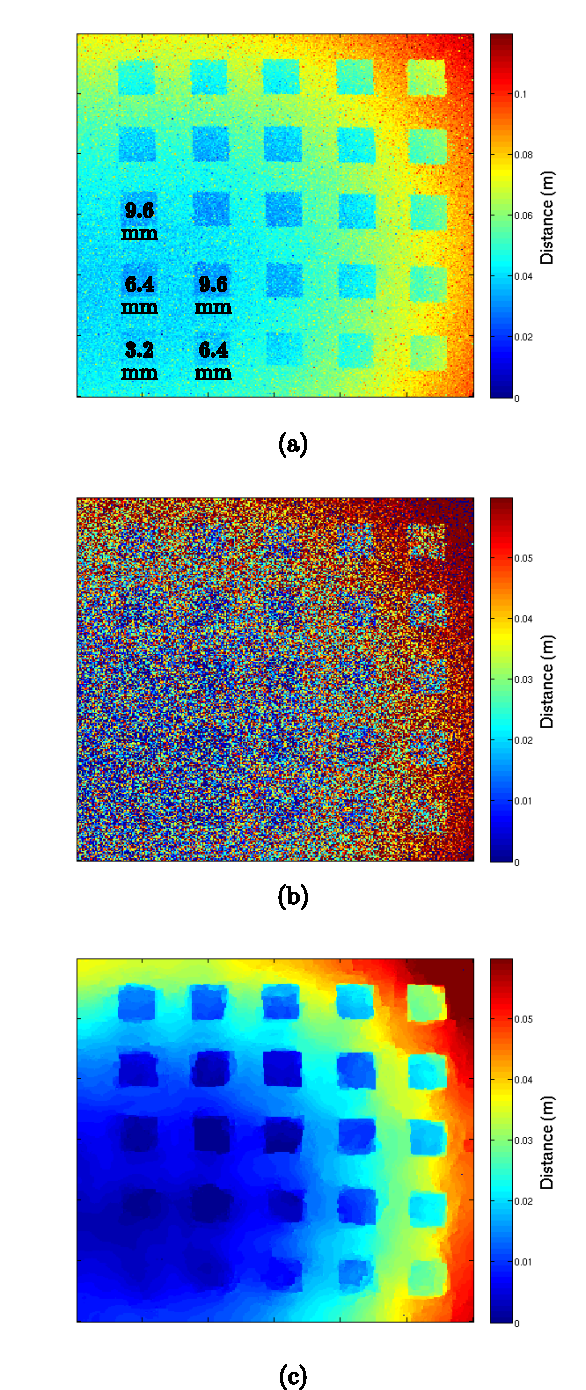
\includegraphics[height=18cm]{figure-first-depthchart.pdf}
\caption{Depth-chart test consisting of square features of linearly increasing height. (a) Image produced by traditional averaging with several hundred detections per pixel, (b) Pixel-wise ML estimate using only the first photon arrival, and (c) data in (b) processed using our computational reconstruction method.}
\label{figure:first-depthchart}
\end{figure}

\subsubsection{Reflectivity chart}

We also constructed a chart to independently analyze the reflectivity-resolving capabilities of our imager. As shown in Figure \ref{figure:first-intensitychart}, the chart consists of printed gray-scale squares arranged in rows of 2, 4, 8, and 16 shades on linear scales, corresponding to 1, 2, 3, and 4 bits of reflectivity resolution, respectively. Figure \ref{figure:first-intensitychart}(a) shows the ground-truth measurement obtained by averaging the number of photon arrivals over a long dwell time. It is essentially a gray-scale photograph in the traditional sense. Figure \ref{figure:first-intensitychart}(b) shows the ML estimate of the reflectivity from only the first photon arrival, which results in an extremely noisy image since the error on the pixel-wise ML estimate is high. Figure \ref{figure:first-intensitychart}(c) shows the same first-photon data processed using our reconstruction technique. We see that we can clearly resolve between 8 and 16 shades of grey, corresponding to $\sim$3 to 4 bits of reflectivity resolution. Again, although it may seem counterintuitive to obtain such high reflectivity resolution using only 1 photon arrival at each pixel, we are exploiting sparsity in the scene and promoting spatially-smooth objects, making use of several nearby pixels of data at once, in contrast to traditional averaging methods which treat each pixel as an independent object.

\begin{figure}[h!]
\centerline{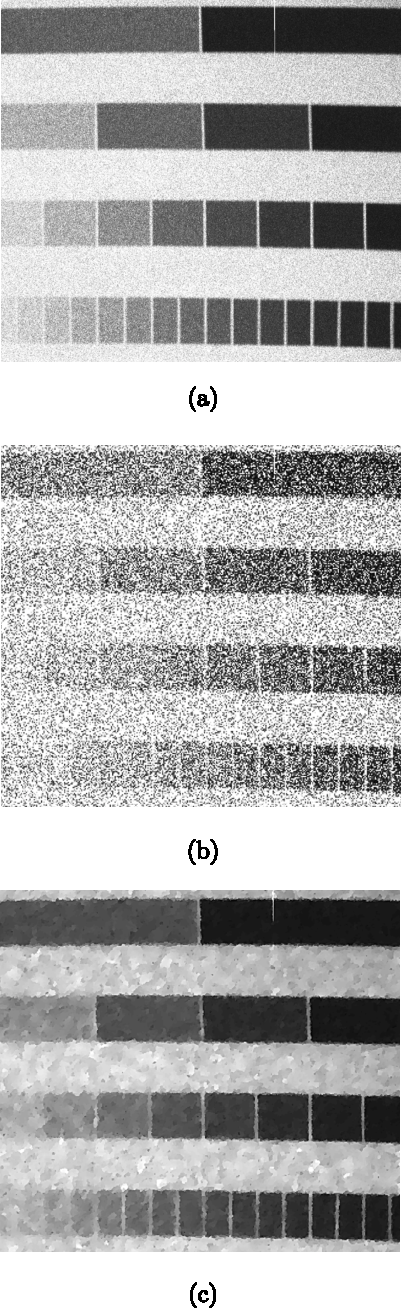
\includegraphics[height=18cm]{figure-first-intensitychart.pdf}}
\caption{Reflectivity-chart test. (a) Image produced by traditional averaging with several hundred detections per pixel, (b) Pixel-wise ML estimate using only the first photon arrival, and (c) data in (b) processed using our computational reconstruction method.}
\label{figure:first-intensitychart}
\end{figure}

\section{Reflectivity from depth data}
We also noted a curious phenomenon in which, in the presence of background noise, the first-photon depth data alone yielded some information about reflectivity without knowledge of the number of pulses until the first detection. We make use of the fact that for pixels in spatially-correlated regions of high reflectivity, signal photons are more likely to reach the detector first, whereas for pixels in regions of low reflectivity, background photons are more likely to reach the detector first. This fact is captured by taking local variances of the depth data; higher variances are the result of first-photon contributions from the uniform time distribution of the background photons, whereas lower variances are the result of increased first-photon contributions from the laser pulse. Figure \ref{figure:first-intensityfromdepth} shows an example of such an image obtained by taking the 1000$\times$1000-pixel raw depth data and estimating each pixel's reflectivity $\alpha(x,y)$ based on the sample variance of the point-wise ML estimates of the arrival times at pixel $(x,y)$ and its eight neighbors:
\begin{equation}
\hat{\alpha}(x,y) = 1 / \sqrt{\operatorname{var}\left(\left\{ Z(x-1, y-1),\,Z(x, y-1),\,Z(x+1,y-1),\,...\, Z(x+1,y+1)\right\}\right)}\,\,.
\end{equation}
Spatial regularization applied to this scheme may be able to further improve the quality of the image; conversely, it may be possible to make use of this additional information in improving the quality of the first-photon images obtained earlier instead of censoring all background detections. It is worth noting that this method of garnering reflectivity data works only in the case in which the background and signal levels are similar; it would not be possible to apply this method to a scenario without background noise.

\begin{figure}[h!]
\centerline{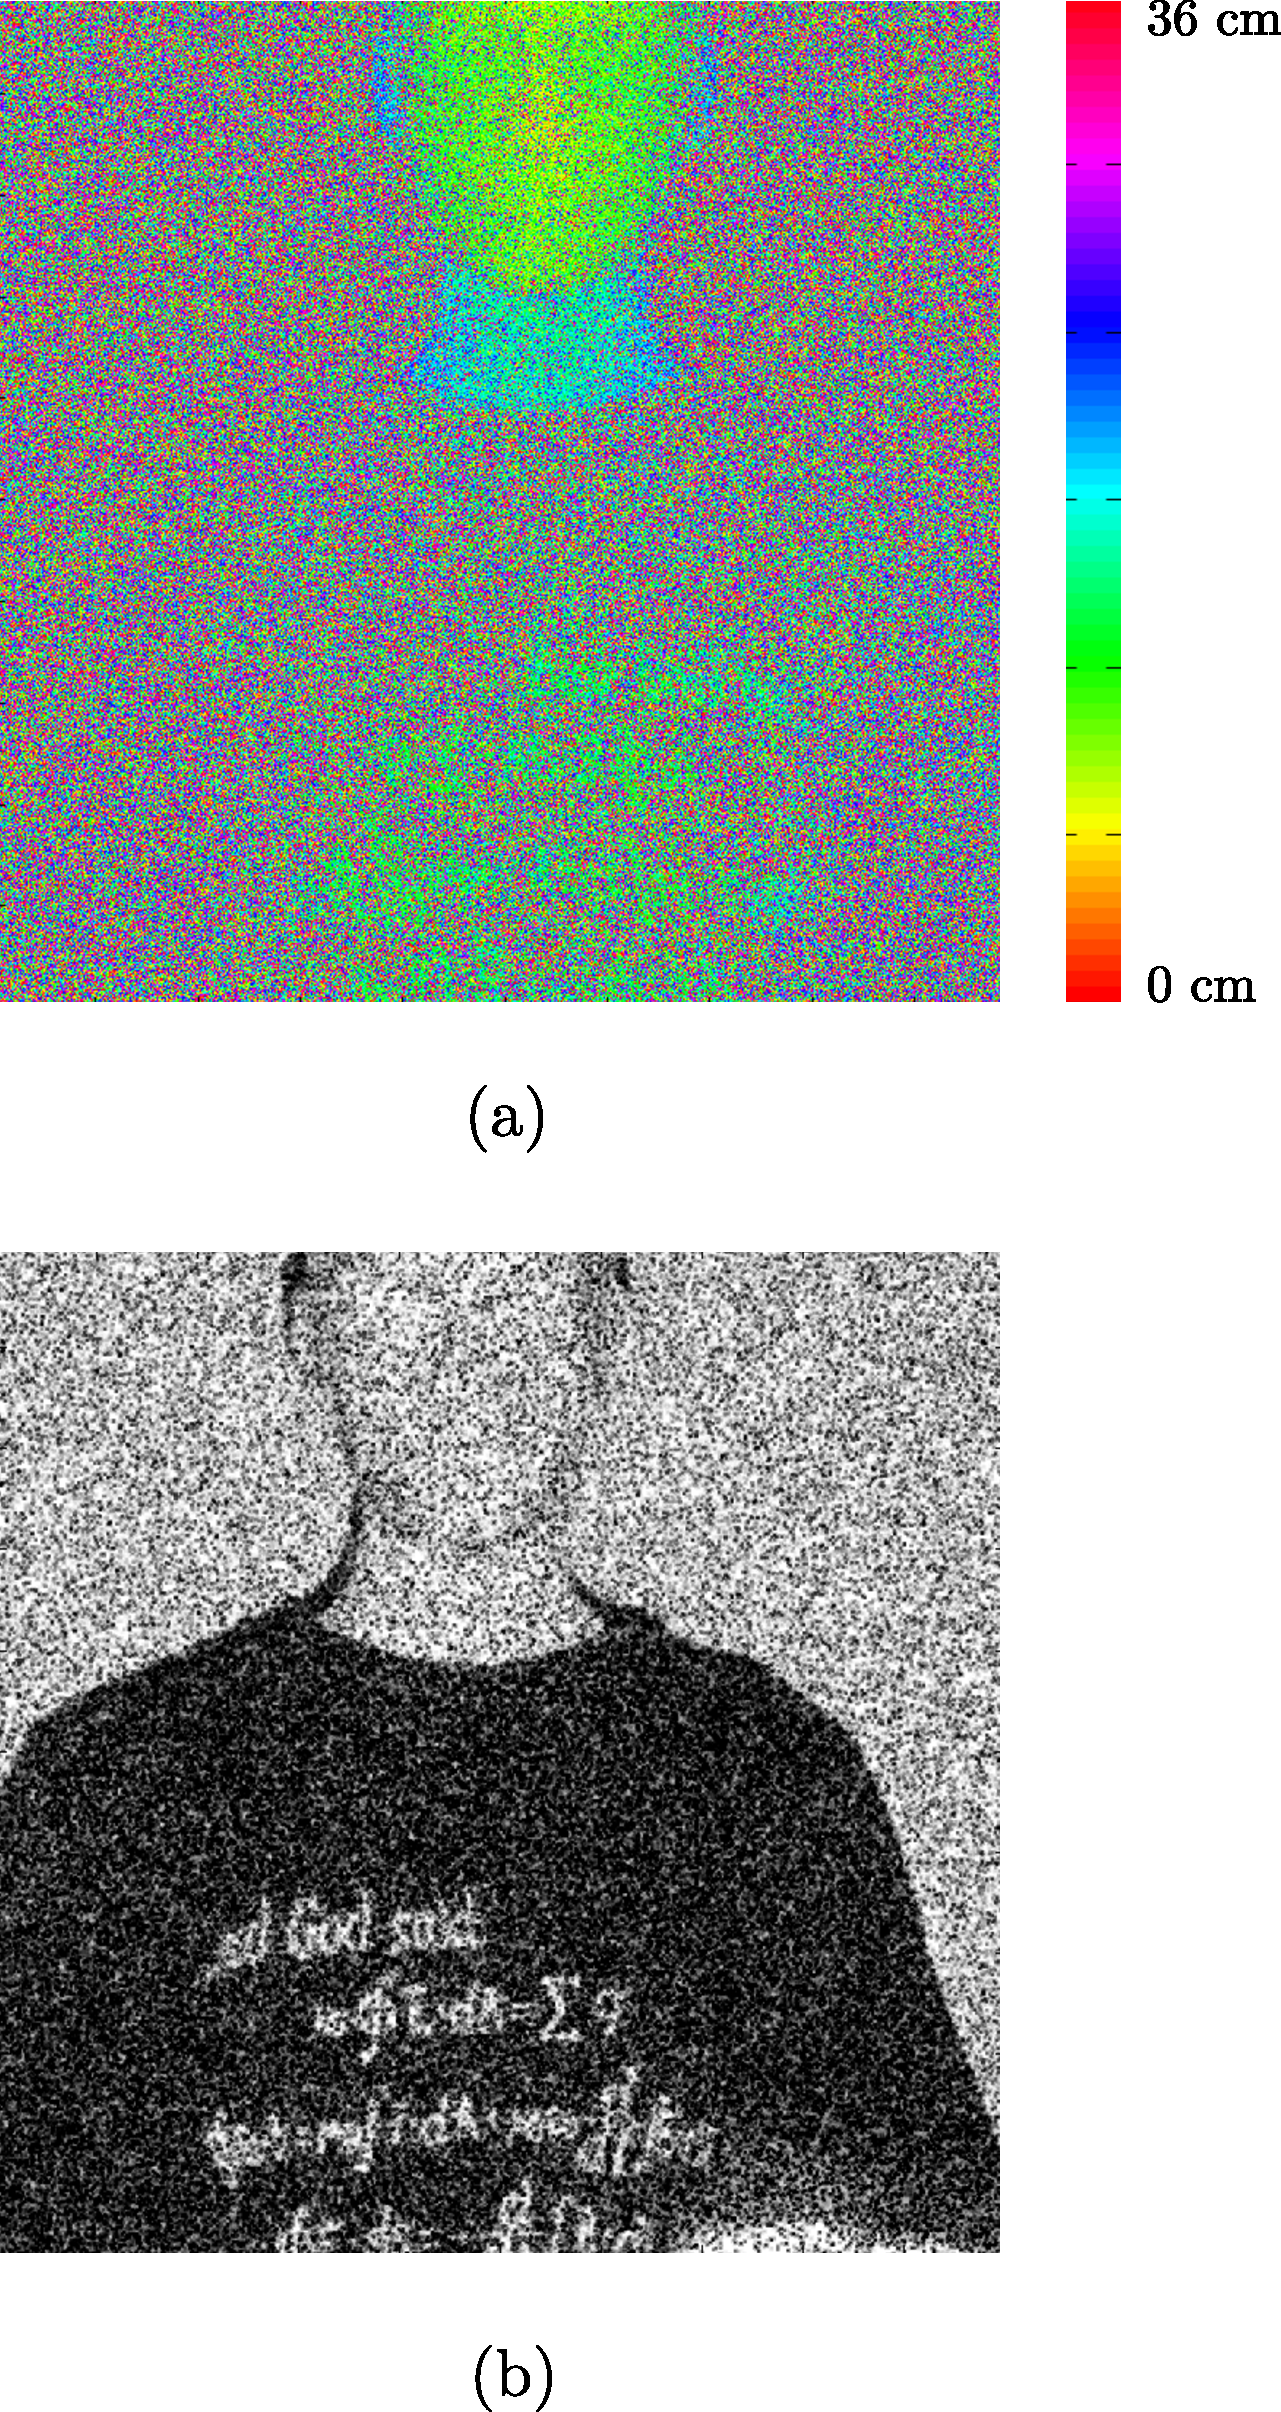
\includegraphics[height=17cm]{figure-first-intensityfromdepth.pdf}}
\caption{(a) Raw depth values from a 1000$\times$1000-pixel first-photon acquisition in the presence of high background noise, but range-gated to the indicated scale for visualization purposes. Evidence of high-reflectivity features on the T-shirt and face visually manifest as coherent regions of color, which are the result of low variances in depth. (b) Reflectivity information gained from a version of (a) without range-gating. The number of pulses until the first detection was not used in this method.}
\label{figure:first-intensityfromdepth}
\end{figure}

\section{Imaging using a SPAD array}

We now turn to the question of single-photon imaging without raster scanning. Arrays of Geiger-mode detectors have not been available until recently, necessitating raster scanning in most single-photon LIDAR experiments. However, it would be highly desirable to be able to image an entire scene in parallel, enabling an acquisition speedup by as much as a factor of the number of pixels and enabling possibilities for real-time high-speed video and other commercial, scientific, or military applications.

Such single-photon avalanche photodiode (SPAD) arrays are currently a popular topic of research. F. Villa et al. at the Politecnico di Milano researched and developed an 32$\times$32-pixel SPAD array \cite{villa-thesis} that features 6-bit photon-counting and 10-bit time-of-flight ranging modes. We formed a collaboration with principal investigator F. Zappa and invited graduate student R. Lussana to bring two prototypes of the SPAD array to MIT to test with our computational reconstruction method.

\subsection{Hardware specifications}
The SPAD array developed by the Zappa group is a 32$\times$32-pixel array of fully independent CMOS SPAD detectors. Each pixel is 150$\times$150 $\mu$m in size, comprising a total array size of 4.8$\times$4.8 mm. Each pixel has a circular active region with diameter 30 $\mu$m, giving a fill factor of 3.14\%. The photon detection efficiency at 640 nm is $\sim$20\% which gives a combined detection efficiency of 0.63\%. Although the efficiency of detection is extremely low, we understand that this is an early-stage prototype device and expect that future research in SPAD arrays will be able to achieve higher fill factors and detection efficiencies. As of this writing, Princeton Lightwave, Inc. \cite{princetonlightwave} has developed commercially-available $128 \times 32$ and $32 \times 32$ InP/InGaAs Geiger-mode APD arrays for operation at $\sim$1064 nm and $\sim$1550 nm.

The dark count rate of the SPAD array is specified at $\sim$100 cps, but we found that in reality the dark count rate varies across pixels. In particular a small number of hot pixels have extremely high dark count rates, which we attribute to the reliability and reproducibility of the fabrication process, as described in \cite{villa-thesis}.

\subsubsection{Modes of operation}

The array has two modes of operation: counting mode and timing mode. In counting mode, the 6-bit registers located at each detector site are incremented each time a photon arrival is detected, allowing for up to 63 photon arrivals (binary 111111) before rolling over to 0. Hence in counting mode it is important to keep the power level low enough to avoid this rollover. Alternatively, in the case of smoothly-varying objects, it may be possible to unwrap the rollover, similar to 1-dimensional phase-unwrapping algorithms.

In timing mode, the SPAD array outputs a digital signal at the start of each acquisition window which can be used to synchronize a laser diode. Figure \ref{figure:first-spad-terms} illustrates the terminology and time scales we will use to describe the timing-mode acquisition process. The 6-bit registers at each pixel are used for recording the time of the first photon arrival at each pixel with a global electronic shutter. An additional 4-bit register at each pixel using a timing interpolation scheme \cite{villa-thesis} provides for a total of 10 bits of timing resolution (1024 bins). The time-bin duration is $\sim$389.9 ps, governed by the hardware clock rate of 160.3 MHz with 16$\times$ multiplication in half-coarse mode \cite{villa-thesis}. Multiplying the time-bin duration by 1024 gives an acquisition window of 399 ns. It should be noted that, unlike our single photon detector and HydraHarp setup, the SPAD array needs additional time for data readout, which takes a minimum of 10 $\mu$s per frame. This limits the maximum frame rate of acquisition to around 100 kfps in burst mode, in which a short number of frames are acquired and data are stored on the SPAD array itself until subsequent offloading to a PC. In continuous acquisition mode, the USB link limits us to an acquisition rate of around 10 kfps.

The acquisition windows being 399 ns, but the length of one frame of data acquisition can be no shorter than 10 $\mu$s, severely impacts our measurement duty cycle. However, the SPAD array also features a refolding mode in which continuous measurements of 1024 time bins (399 ns) are performed back-to-back in a single frame but without resetting the registers; whenever a photon is detected at a particular pixel, that pixel will no longer record any more data until the registers are reset at the start of next frame. However, to avoid overheating, it was helpful to maintain the active acquisition duty cycle (gate-on time) under $1/4$. In our measurements, we used this refolding-mode acquisition, extending the frame length to 65 $\mu$s and acquiring continuously in for 16 $\mu$s within that 65 $\mu$s. The remaining 49 $\mu$s is used for cool-off and data transfer.

The SPAD array also includes a feature that enables multiple laser pulses to be fired within each acquisition window. Since our 1024-bin, 399-ns acquisition window is much larger than our laboratory in speed-of-light units, we configured the SPAD array to fire 8 laser pulses per window (i.e., one pulse per 128 time bins).

Note that in refolding mode the SPAD hardware does not reset any registers until a readout, and thus does not provide information about which pulse a particular photon detection corresponds to. Thus, for reflectivity measurements it is important to ensure that the refolding factor is low enough that we are not saturating each pixel with a photon at every frame. If most of the 32$\times$32 pixels register detections at each frame, our ML reflectivity estimates would be featureless and it would be impossible to use Poisson statistics to infer any information. (An alternate approach would be to simply switch the SPAD array to counting mode to perform reflectivity measurements. However, changing the SPAD acquisition mode is not instantaneous and requires reprogramming the on-board FPGA, thus making high-speed alternating acquisition impossible with the current hardware design.)

\subsection{Experimental setup}
A diagram of the experimental setup is shown in Figure \ref{figure:first-spad-setup}. The illumination used the same PicoQuant LDH-series laser but configured for flood illumination using two ground-glass diffusers in series (one single layer preserved too much coherence and created large-size speckles on the target). The laser diode was operated in external clock mode, driven by the laser trigger output of the SPAD array.
 
\begin{figure}[h!]
\centerline{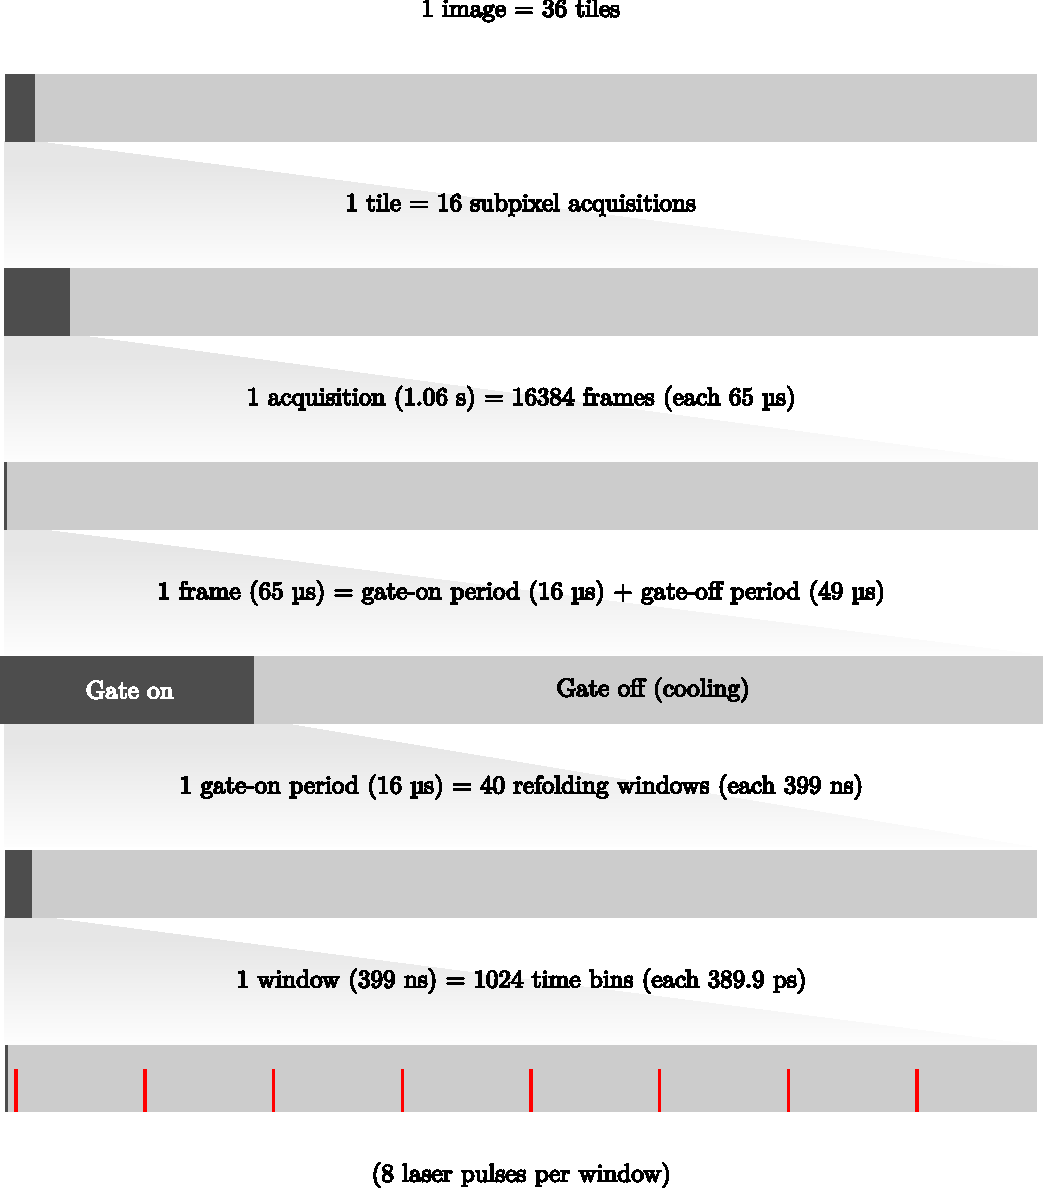
\includegraphics[width=15cm]{figure-first-spad-terms.pdf}}
\caption{Terminology used in the describing the SPAD array imaging acquisition scheme.}
\label{figure:first-spad-terms}
\end{figure}

The SPAD array has a total array size of 4.8$\times$4.8 mm with 32$\times$32 pixels. In principle we would like both a larger imaging area as well as a higher number of pixels in order to experiment with computational reconstruction methods. Given the limited size of the current SPAD array, we opted to use multiple image scans to form a larger-size composite image. We mounted the SPAD array on a feedback-controlled, two-axis motorized translation stage and translated over exactly 6$\times$6 tiles of the 4.8$\times$4.8 mm array, as shown in Figure \ref{figure:first-spad-scanning}(a), giving us a total imaging area of 28.8$\times$28.8 mm and a resolution of 192$\times$192 pixels. However, since the active area of each pixel is only 30 $\mu$m in diameter, which is less than 1/4 of the pixel pitch, we were able to multiply this resolution through factor-of-4 subsampling at each pixel, translating the SPAD array along both axes to all combinations of fractional pixel pitch distances (0, 1/4, 1/2, and 3/4) along both $x$- and $y$-axes before moving onto the next tile, as shown in Figure \ref{figure:first-spad-scanning}(b)-(d). In other words, we translated the SPAD array to all combinations of positions $(x, y) = (L_i + \Delta_j, L_k + \Delta_l)$ for all combinations of $L_i, L_k \in \{ 0, 4.8, 9.6, 14.4, 19.2, 24\}$ (tile positions) and $\Delta_j, \Delta_k \in \{ 0, .0375, .0750, .1125\}$ (subpixel sampling) where all dimensions are in mm. This gave us a total imaging resolution of $32 \times 5 \times 4$ = $768$ pixels along each axis and required a total of $5 \times 5 \times 4 \times 4$ = 400 total acquisitions to produce a resulting $768\times 768$ image. Although this required scanning, it was still significantly faster than raster scanning over single pixels, which would have required a total of $768^2 = 518400$ acquisitions for the same resolution image.

In order to obtain sufficient data for future analysis work in the short period of time with the SPAD array in our laboratory, we configured the SPAD to output a total of 16384 frames of data for each acquisition, which at 65 $\mu$s per frame took 1.06 seconds. The MATLAB user interface for the SPAD array was modified to automate the acquisition procedure and synchronously drive the translation stages to each of the 400 positions, outputting a separate data file for each position containing photon arrival data.

\begin{figure}[h!]
\centerline{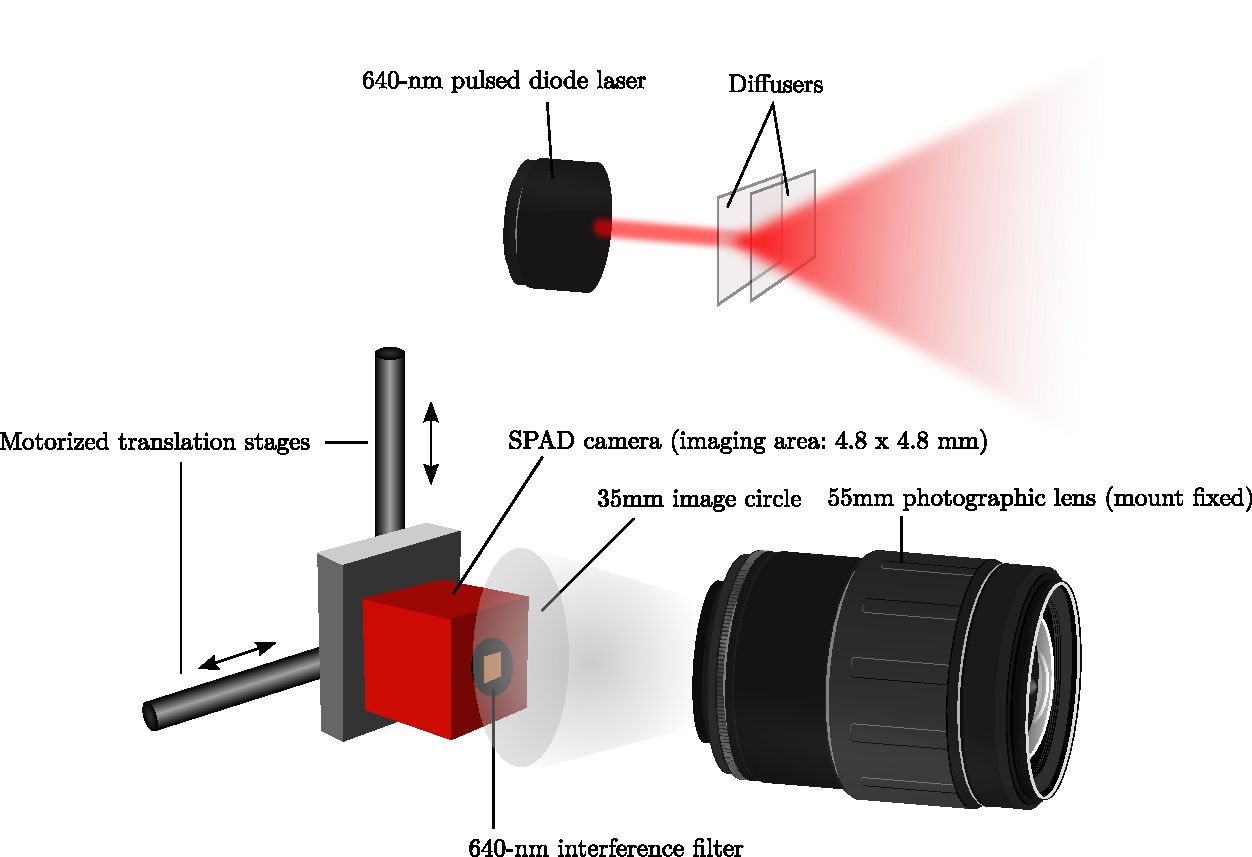
\includegraphics[width=\textwidth]{figure-first-spad-setup.pdf}}
\caption{Experimental setup for single-photon imaging with a SPAD array.}
\label{figure:first-spad-setup}
\end{figure}

The original software for the SPAD array was configured to output the values of all SPAD registers at each acquisition frame, even in the event of no photon arrivals. However, since we operate in a low-flux regime, where in any given frame most pixels do not contain arrival data, this is an inefficient method of data storage, with each single acquisition occupying several gigabytes. In addition, the output of the SPAD array pixel data is not in logical pixel order due to limitations in the design of the electronics \cite{villa-thesis}. In order to speed up data processing, we developed a custom GNU C program (see Appendix \ref{appendix:spadcounts}) to read the SPAD array binary files and output a cleaner, MATLAB-friendly file containing only a sequence of photon detections tagged by pixel number and time frame number. The C program also has both ASCII and binary output modes, that are conveniently and efficiently readable in MATLAB.

Mounted in front of the translatable SPAD array was a standard Canon FL-series photographic lens with a focal length of 55 mm and a maximum photographic aperture of f/1.2. We set the aperture of the lens to f/2.8 which provided the necessary depth of field to capture sufficient detail from various depths of our object, increase sharpness, and reduce vignetting. The lens, designed for 35 mm film cameras, had an image circle of slightly larger than 35 mm, allowing us to mount the lens at a fixed position and conveniently fit our $24\times24$ mm square imaging area entirely within the image circle of the lens. Basic tests in counting mode showed that at f/2.8, the lens was able to easily and clearly resolve objects as small as one single pixel in the $768\times768$ pixel image with almost zero cross-talk, provided that the lens was manually focused correctly.

\begin{figure}[h!]
\centerline{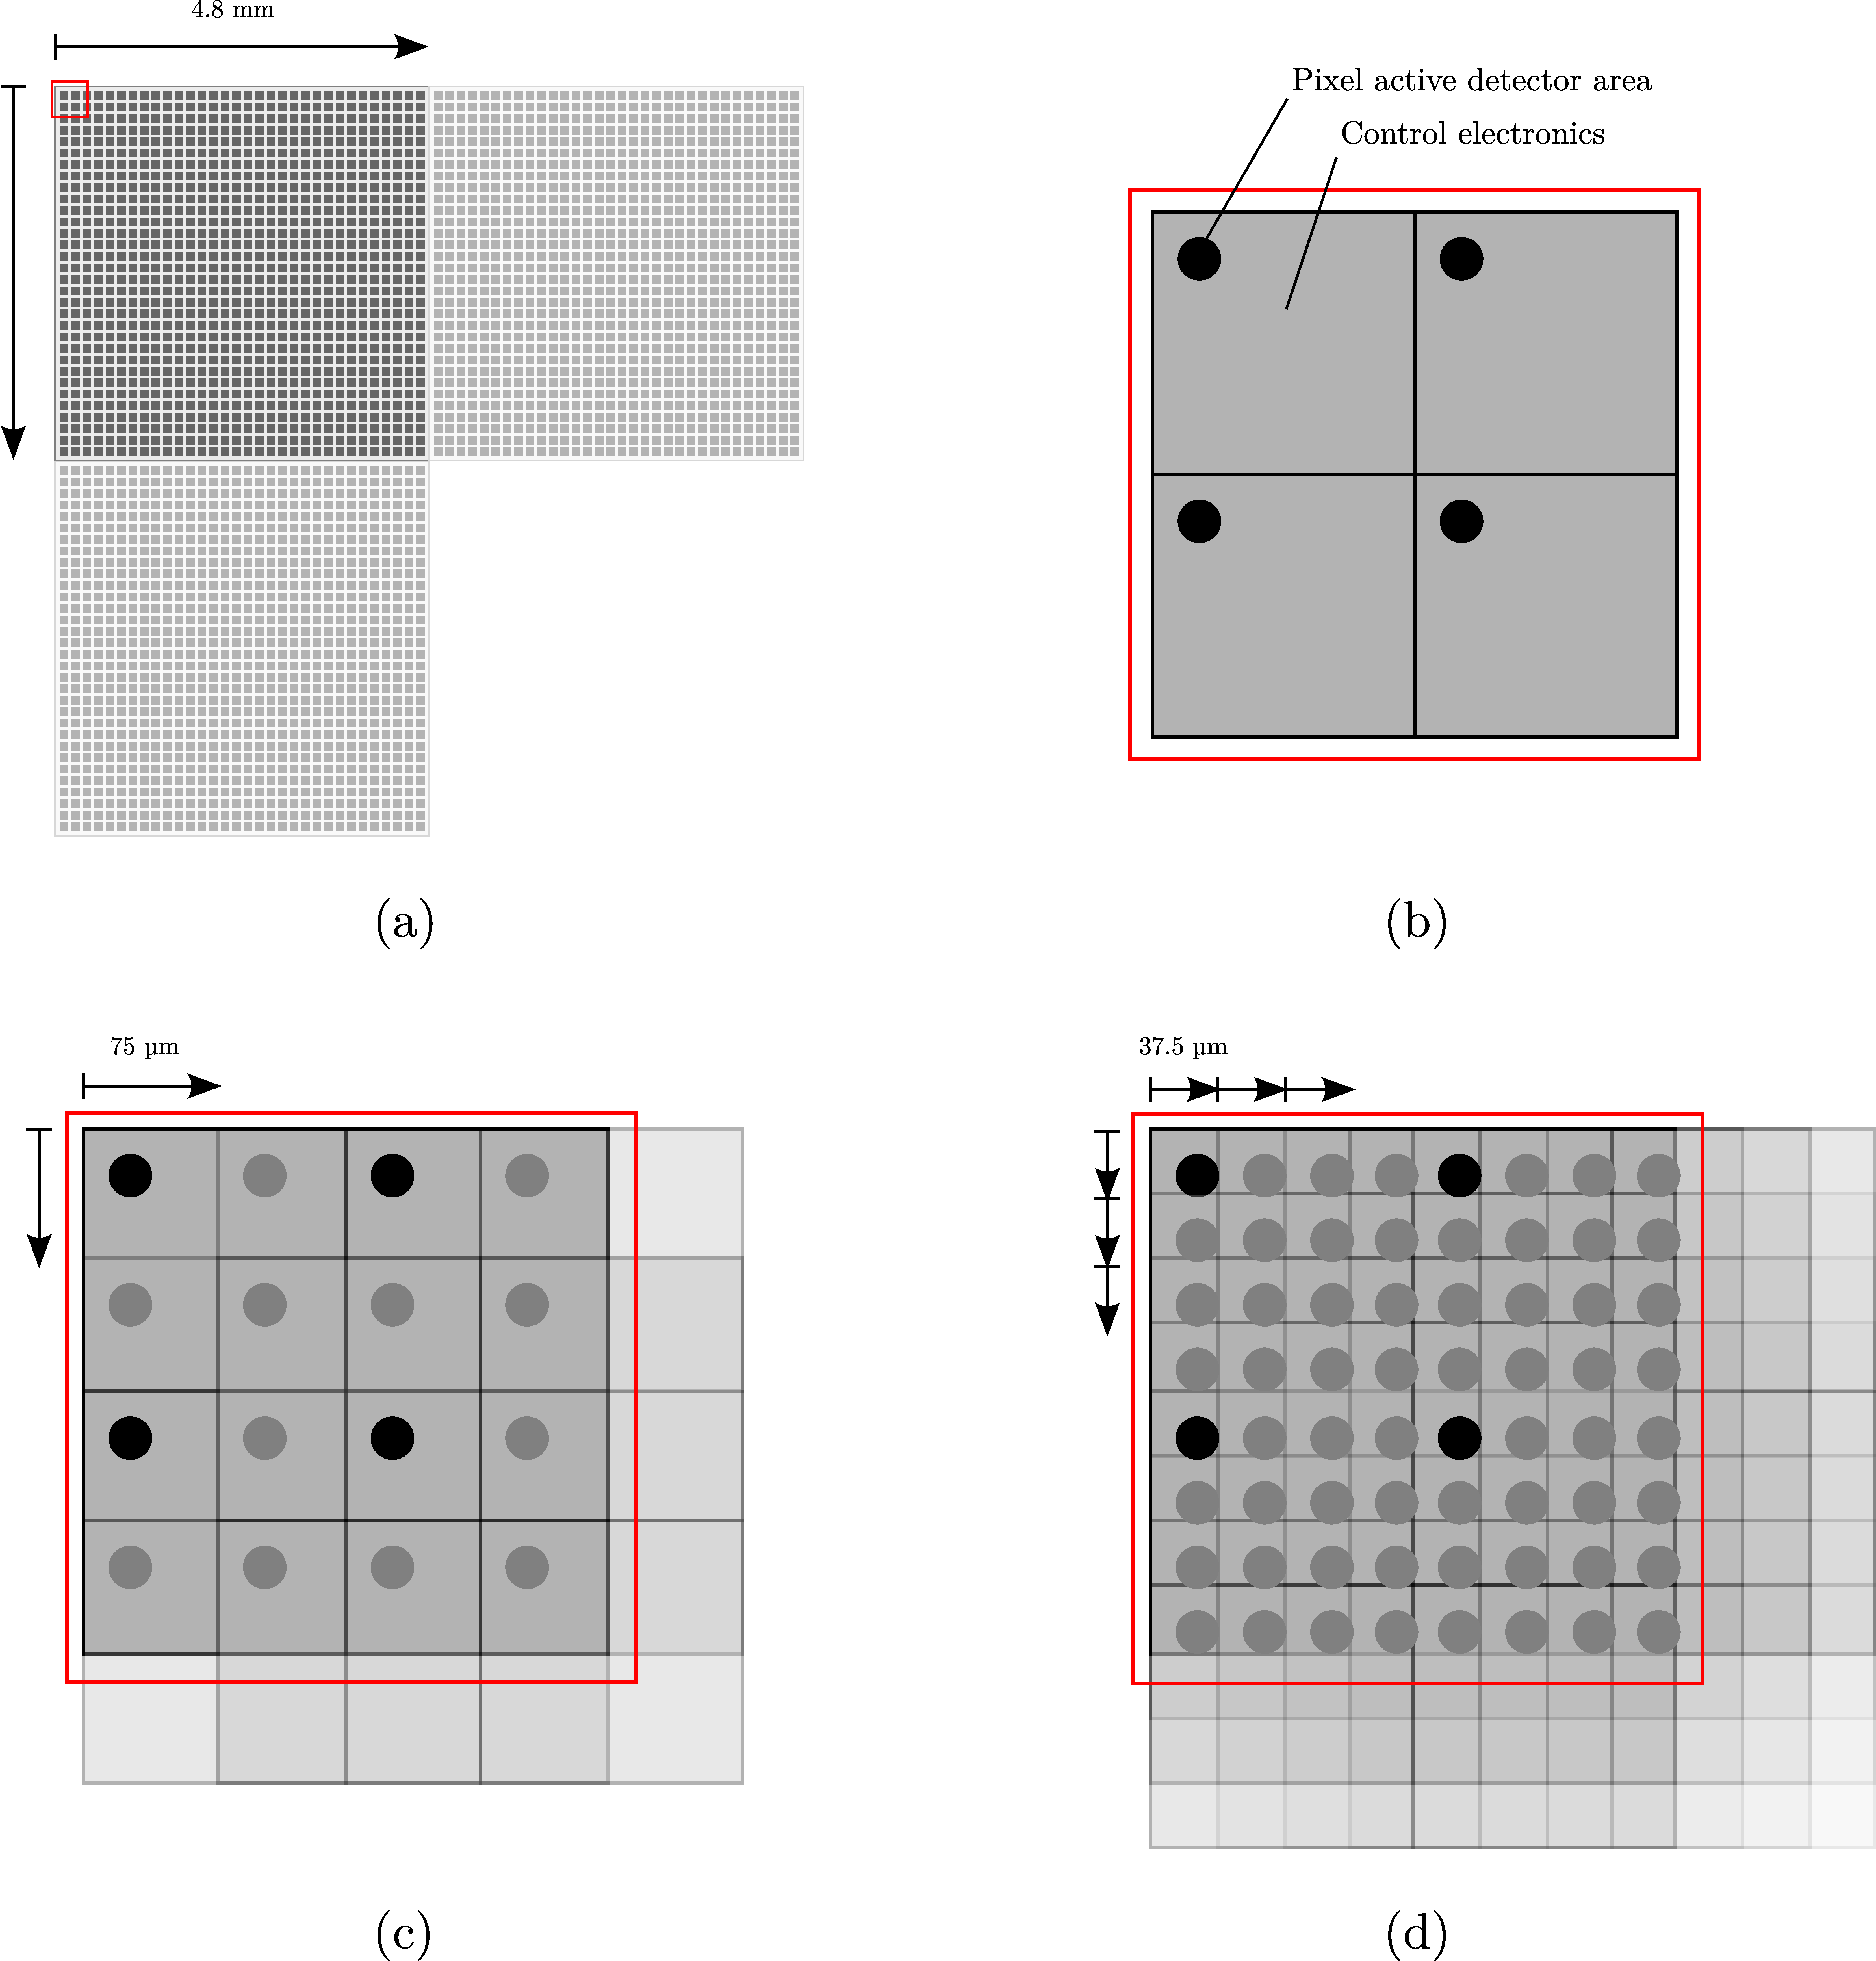
\includegraphics[width=15cm]{figure-first-spad-scanning.pdf}}
\caption{Scanning scheme to obtain high-resolution images using the 32$\times$32-pixel SPAD array. (a) We translate the array by increments of a full array size (4.8 mm) along both axes to image multiple "tiles" of the entire array. (b) Zoom-in view of individual SPAD pixels showing the active area with no subpixel scanning, (c) 2$\times$2 subpixel scanning by translating along each axis by 75 $\mu$m, multiplying the resolution by 2 and (d) 4$\times$4 subpixel scanning by translating along each axis by 37.5 $\mu$m, 75 $\mu$m, and 112.5 $\mu$m, multiplying the resolution by 4.}
\label{figure:first-spad-scanning}
\end{figure}


\subsection{Computational reconstruction approach}

Unlike first-photon imaging in which the protocol guarantees an arrival at every pixel, single-photon imaging using a SPAD array must use a single deterministic dwell time for the entire image. This has the following implications: for very dark regions it is possible that no photon arrivals will be measured (unlike first-photon imaging where an arrival is guaranteed by definition), while on the other hand, it is also possible that for bright regions, multiple arrivals will be measured in one dwell time period which can be used to gain additional information. Shin et. al. \cite{kirmani-photon} adapted the three-step algorithm from first-photon imaging to be applicable to the fixed-dwell time case, as summarized below.

\subsubsection{Reflectivity reconstruction}
In first-photon imaging we reconstruct reflectivity using the number of laser pulses $n(x,y)$ before the first detected photon and the fact that the maximum-likelihood estimate of the reflectivity using this information is proportional to $1/n$ based on Poisson statistics. In the case of a fixed dwell time of $N$ laser pulses per pixel, we simply measure the total number of photon detections $k(x,y)$ for each pixel and set adjust our negative log-likelihood function to
\begin{equation}
\mathcal{L}\left( \alpha(x,y) | k(x,y) \right) = \gamma \left[ \alpha(x,y) S + B T_r \right] \left[ N - k(x,y) \right] - k(x,y) \log \left[ 1 - \exp \left[ - \gamma \alpha(x,y) S + B T_r \right] \right]\,\,.
\label{equation:spad-ref-ll}
\end{equation}
This function is also strictly convex in $\alpha(x,y)$ and we proceed normally using the same computational reconstruction program for $\hat{\alpha}(x,y)$ using the modified negative log-likelihood from Eq. \ref{equation:spad-ref-ll}.

\subsubsection{Background count rejection}
Since for each pixel we obtain not exactly one arrival, but anywhere from $0$ to $N$ arrivals (in the low-flux regime we neglect the possibility that multiple arrivals occur in a single laser pulse), our background censoring needs to be adjusted accordingly. Shin et. al. \cite{kirmani-photon} suggest that given a set of arrivals $\left\{ t_\ell(x,y) \right\}$ at pixel $(x,y)$, we compute the rank-ordered mean (ROM) $t_{ROM}(x,y)$ which is the median value of the detection times of all the detections acquired in the neighboring 8 pixels, setting $t_{ROM}(x,y) = \infty$ in the case of missing data. The set of indices of uncensored detections $U(x,y)$ at pixel $(x,y)$ is then defined by
\begin{equation}
U(x,y) = \left\{ \ell : |t_\ell(x,y) - t_{ROM}(x,y)| < 2 T_p \left( \frac{BT_r}{\gamma \alpha(x,y)S + BT_r}  \right), 0 \leq \ell \leq k(x,y) \right\}\,\,.
\end{equation}
Similar to first-photon imaging, this procedure is dependent on the reflectivity estimate $\hat{\alpha}(x,y)$ obtained from the result of the optimization in the first step.

\subsubsection{Depth reconstruction}
We now proceed to depth reconstruction. If $U(x,y)$ is non-empty, we set the negative log-likelihood function for depth reconstruction by summing over the log likelihoods of all uncensored detections:
\begin{equation}
\mathcal{L}\left( Z(x,y) | \left\{t_\ell(x,y) | \ell \in U(x,y) \right\} \right) = - \sum_{\ell \in U(x,y)} \log\left[ s(t_\ell(x,y) - \frac{2Z(x,y)}{c}) \right]\,\,.
\end{equation}
If $U(x,y)$ is empty, i.e., if after background censoring, no data is available for pixel $(x,y)$, we set the value of the log-likelihood function to $0$ so that it does not contribute to the scene's overall log-likelihood cost function \cite{kirmani-photon}. We then proceed with the optimization program for $\hat{Z}(x,y)$ as before. Implementation of the optimization procedures for fixed dwell time imaging was also performed using the SPIRAL-TAP package for MATLAB.

\subsection{Preliminary results}

Figures \ref{figure:first-spad-pvnrt-i} shows the reflectivity-imaging results of our reconstruction approach for data taken with the same mannequin used for first-photon imaging but wearing a T-shirt with larger text and a colored background. Figures \ref{figure:first-spad-boxbooks-i} and \ref{figure:first-spad-bball-i} show reflectivity-imaging results from two other scenes among several that were imaged. Although we took data with full 4$\times$4 subpixel scans (768$\times$768 total image pixels), for this thesis we only analyzed data from 2$\times$2 subscans (384$\times$384) because in the full subscan data hot pixels appear in groups of 4$\times$4. Hot pixels interfere with our sparsity-promoting regularization as they effectively get recognized and emphasized as 4$\times$4-pixel features. A more advanced algorithm may be able to specifically recognize and mitigate this situation by performing aggressive range gating based on nearby pixel data when a 4$\times$4-pixel group of hot pixels is detected.

\subsection{Comparison to first-photon imaging}

We notice that for the reflectivity measurements, we see that similar to first-photon imaging, we obtain cleaner images. However unlike first-photon imaging, the dynamic range of reflectivity measurements using the SPAD array is more limited. If we tune the dwell time such that the bright regions receive on the order of $\sim$1-5 photons, we obtain almost no data for darker regions (including, for example, the black background cloth behind the mannequin) because the lack of any signal photon arrivals prevents us from gaining any information about reflectivity variations. This is in stark contrast to first-photon imaging in which an arrival at each pixel is guaranteed by definition (each pixel has a variable dwell time that ends upon a detection event). If we extend the dwell time long enough such that we receive at least one arrival for most pixels, we obtain clean images, but in this case there are sufficient arrivals in the bright regions to obtain excellent results by simply using traditional averaging with excellent results, hence reducing the need for a sparsity-based approach to reconstruct reflectivity images.

The level of improvement obtained in fixed dwell time reflectivity imaging is much less than that of first-photon imaging. We also confirmed this behavior by post-proccessing data from the SPAD arrays to simulate first-photon imaging, in which we gather data for an extended period of time but only keep the first photon arrival at every pixel. The results, shown in Figure \ref{figure:first-spad-first-i} for two scenes, demonstrate again the level of improvement seen using the raster scanning equipment earlier, including the ability to recover text that is almost illegible from the pixel-wise ML estimates.

Shin et al. \cite{kirmani-photon} attempted the reverse, i.e., simulating a SPAD array by taking extended data from the first-photon imager and operating on data acquired within a fixed dwell time at each pixel. The results show a greater degree of improvement than is seen using our real SPAD array, which prompts future investigation. One possibility in explaining this discrepancy may be the non-uniform background count levels in the hardware SPAD array, caused by fabrication inconsistencies, which are not accounted for in the modified reconstruction above.

\begin{figure}[h!]
\centerline{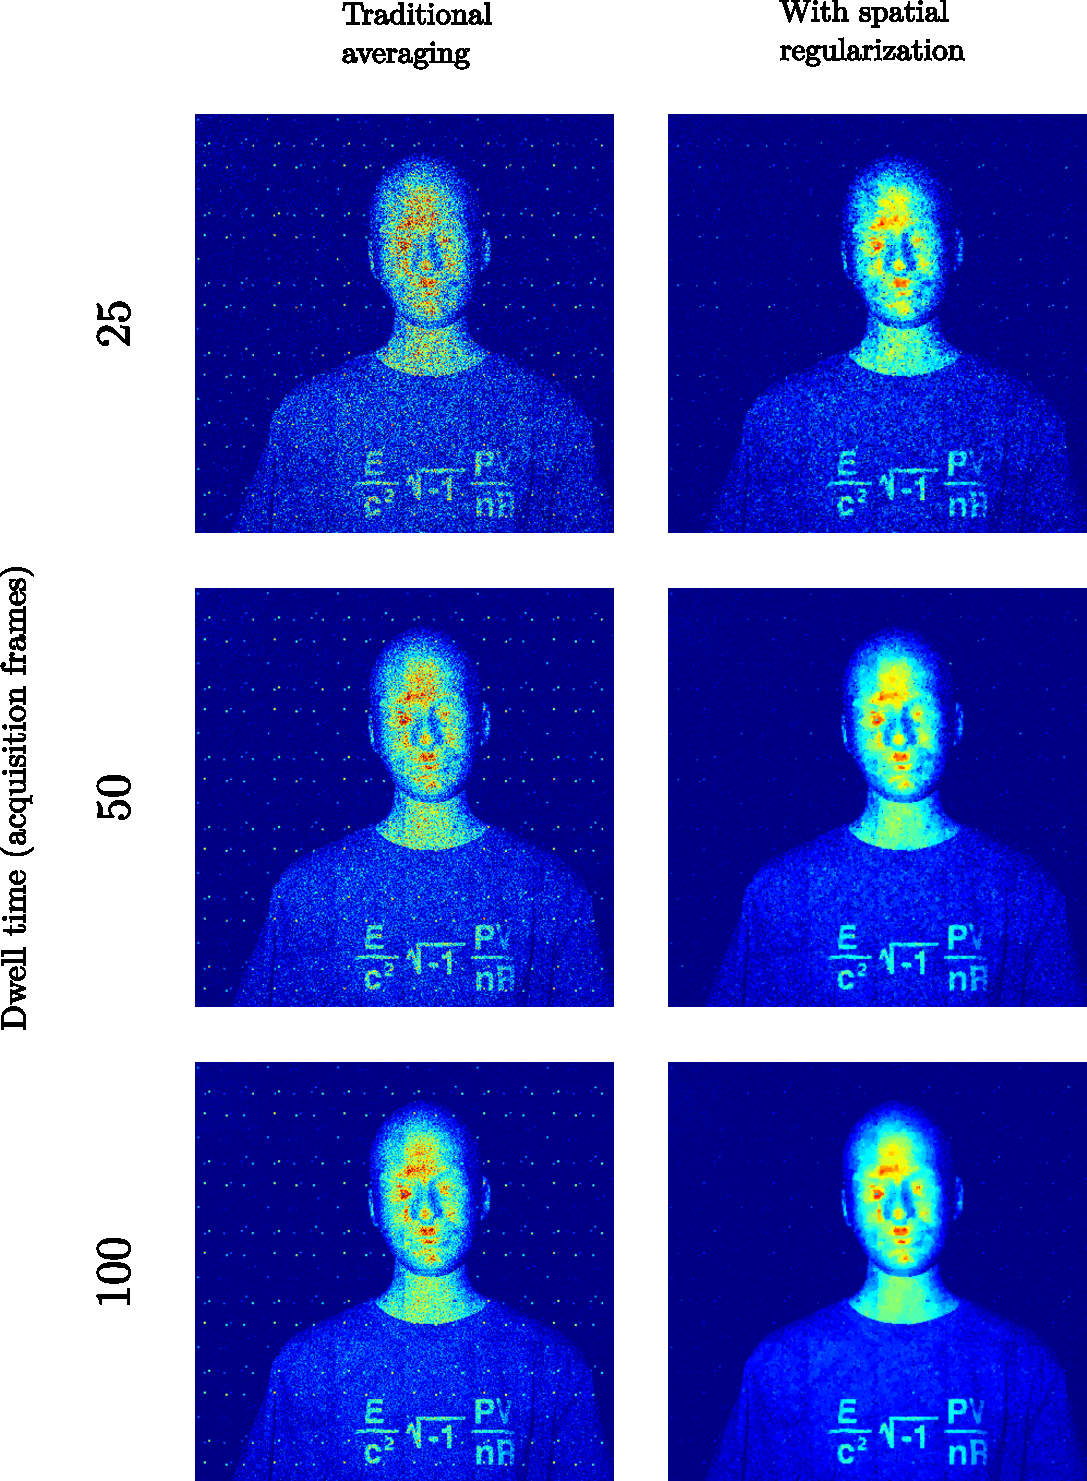
\includegraphics[width=15cm]{figure-first-spad-pvnrt-i.pdf}}
\caption{SPAD array imaging results for 360$\times$360-pixel reflectivity images of a mannequin comparing traditional averaging with spatial regularization. Dwell times are in time units of acquisition frames (65 $\mu$s).}
\label{figure:first-spad-pvnrt-i}
\end{figure}

\begin{figure}[h!]
\centerline{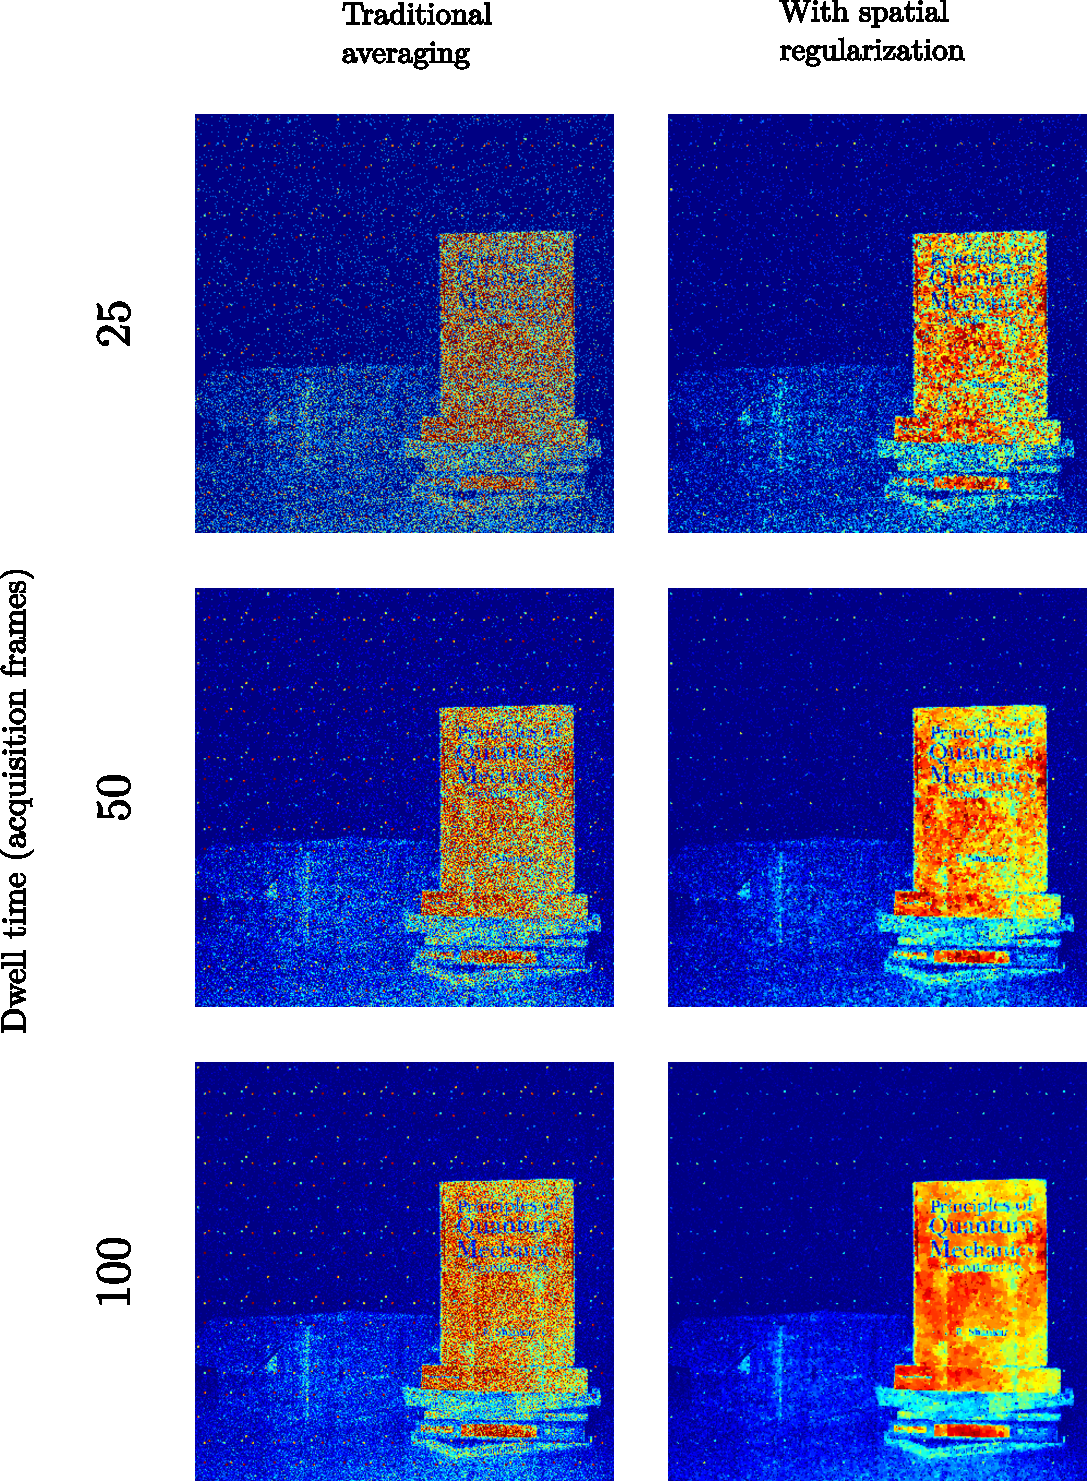
\includegraphics[width=15cm]{figure-first-spad-boxbooks-i.pdf}}
\caption{SPAD array imaging results for 360$\times$360-pixel reflectivity images of a table, cardboard box, and books comparing traditional averaging with spatial regularization. Dwell times are in time units of acquisition frames (65 $\mu$s).}
\label{figure:first-spad-boxbooks-i}
\end{figure}

\begin{figure}[h!]
\centerline{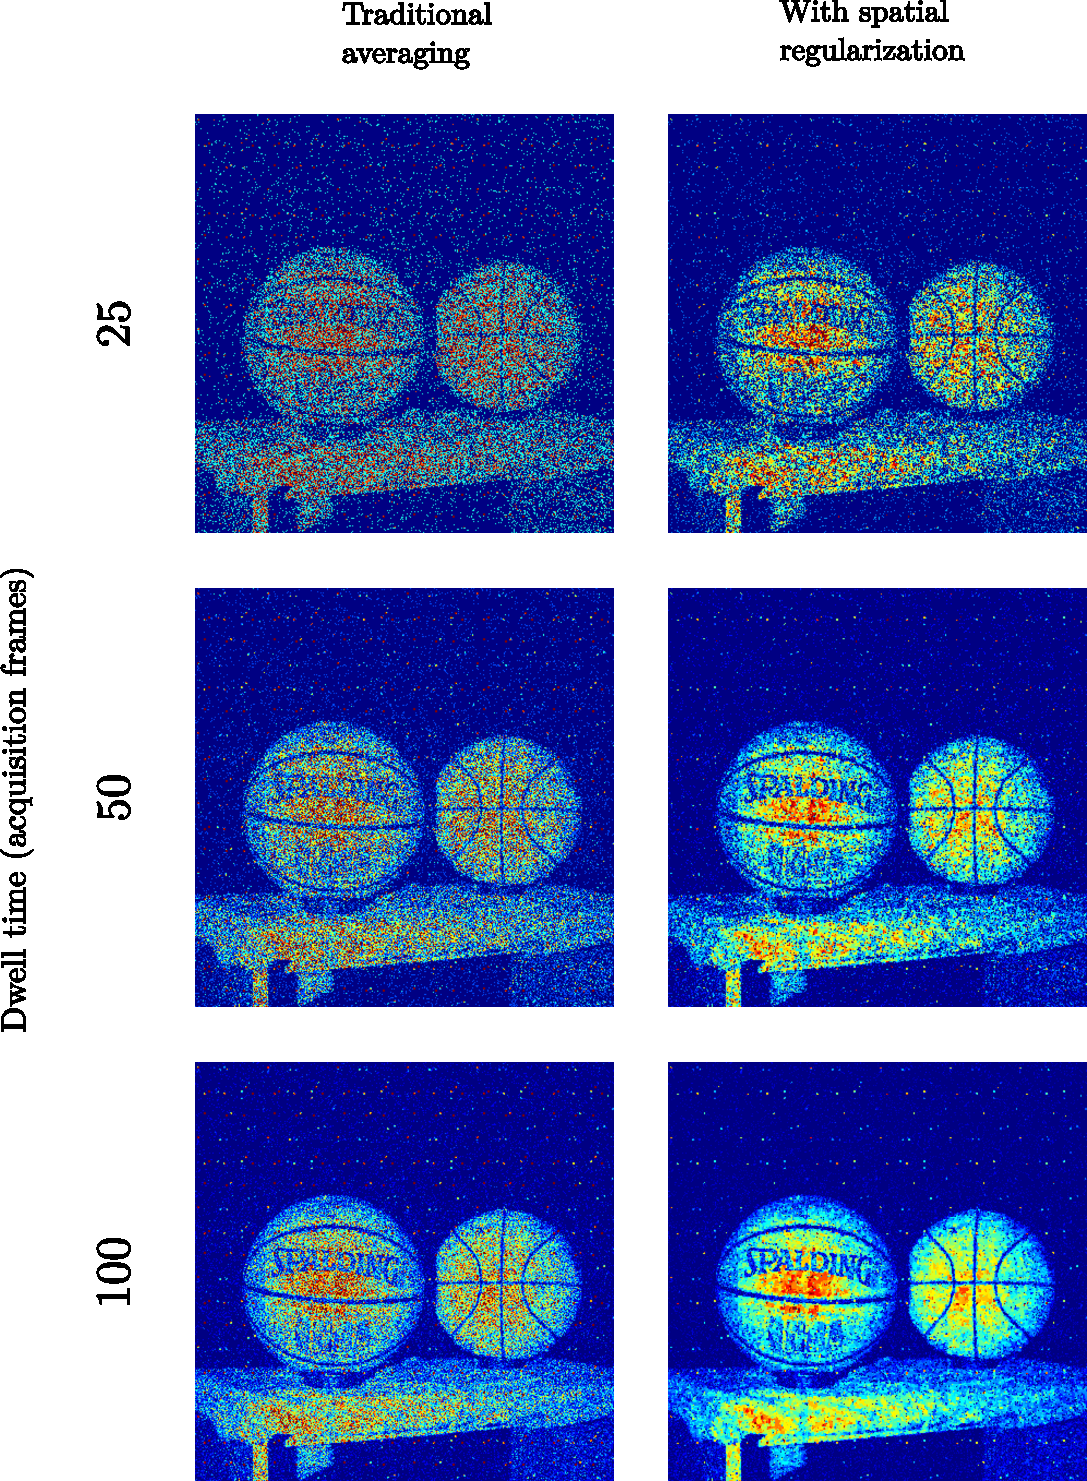
\includegraphics[width=15cm]{figure-first-spad-bball-i.pdf}}
\caption{SPAD array imaging results for 360$\times$360-pixel reflectivity images of two basketballs comparing traditional averaging with spatial regularization. Dwell times are in time units of acquisition frames (65 $\mu$s).}
\label{figure:first-spad-bball-i}
\end{figure}

\begin{figure}[h!]
\centerline{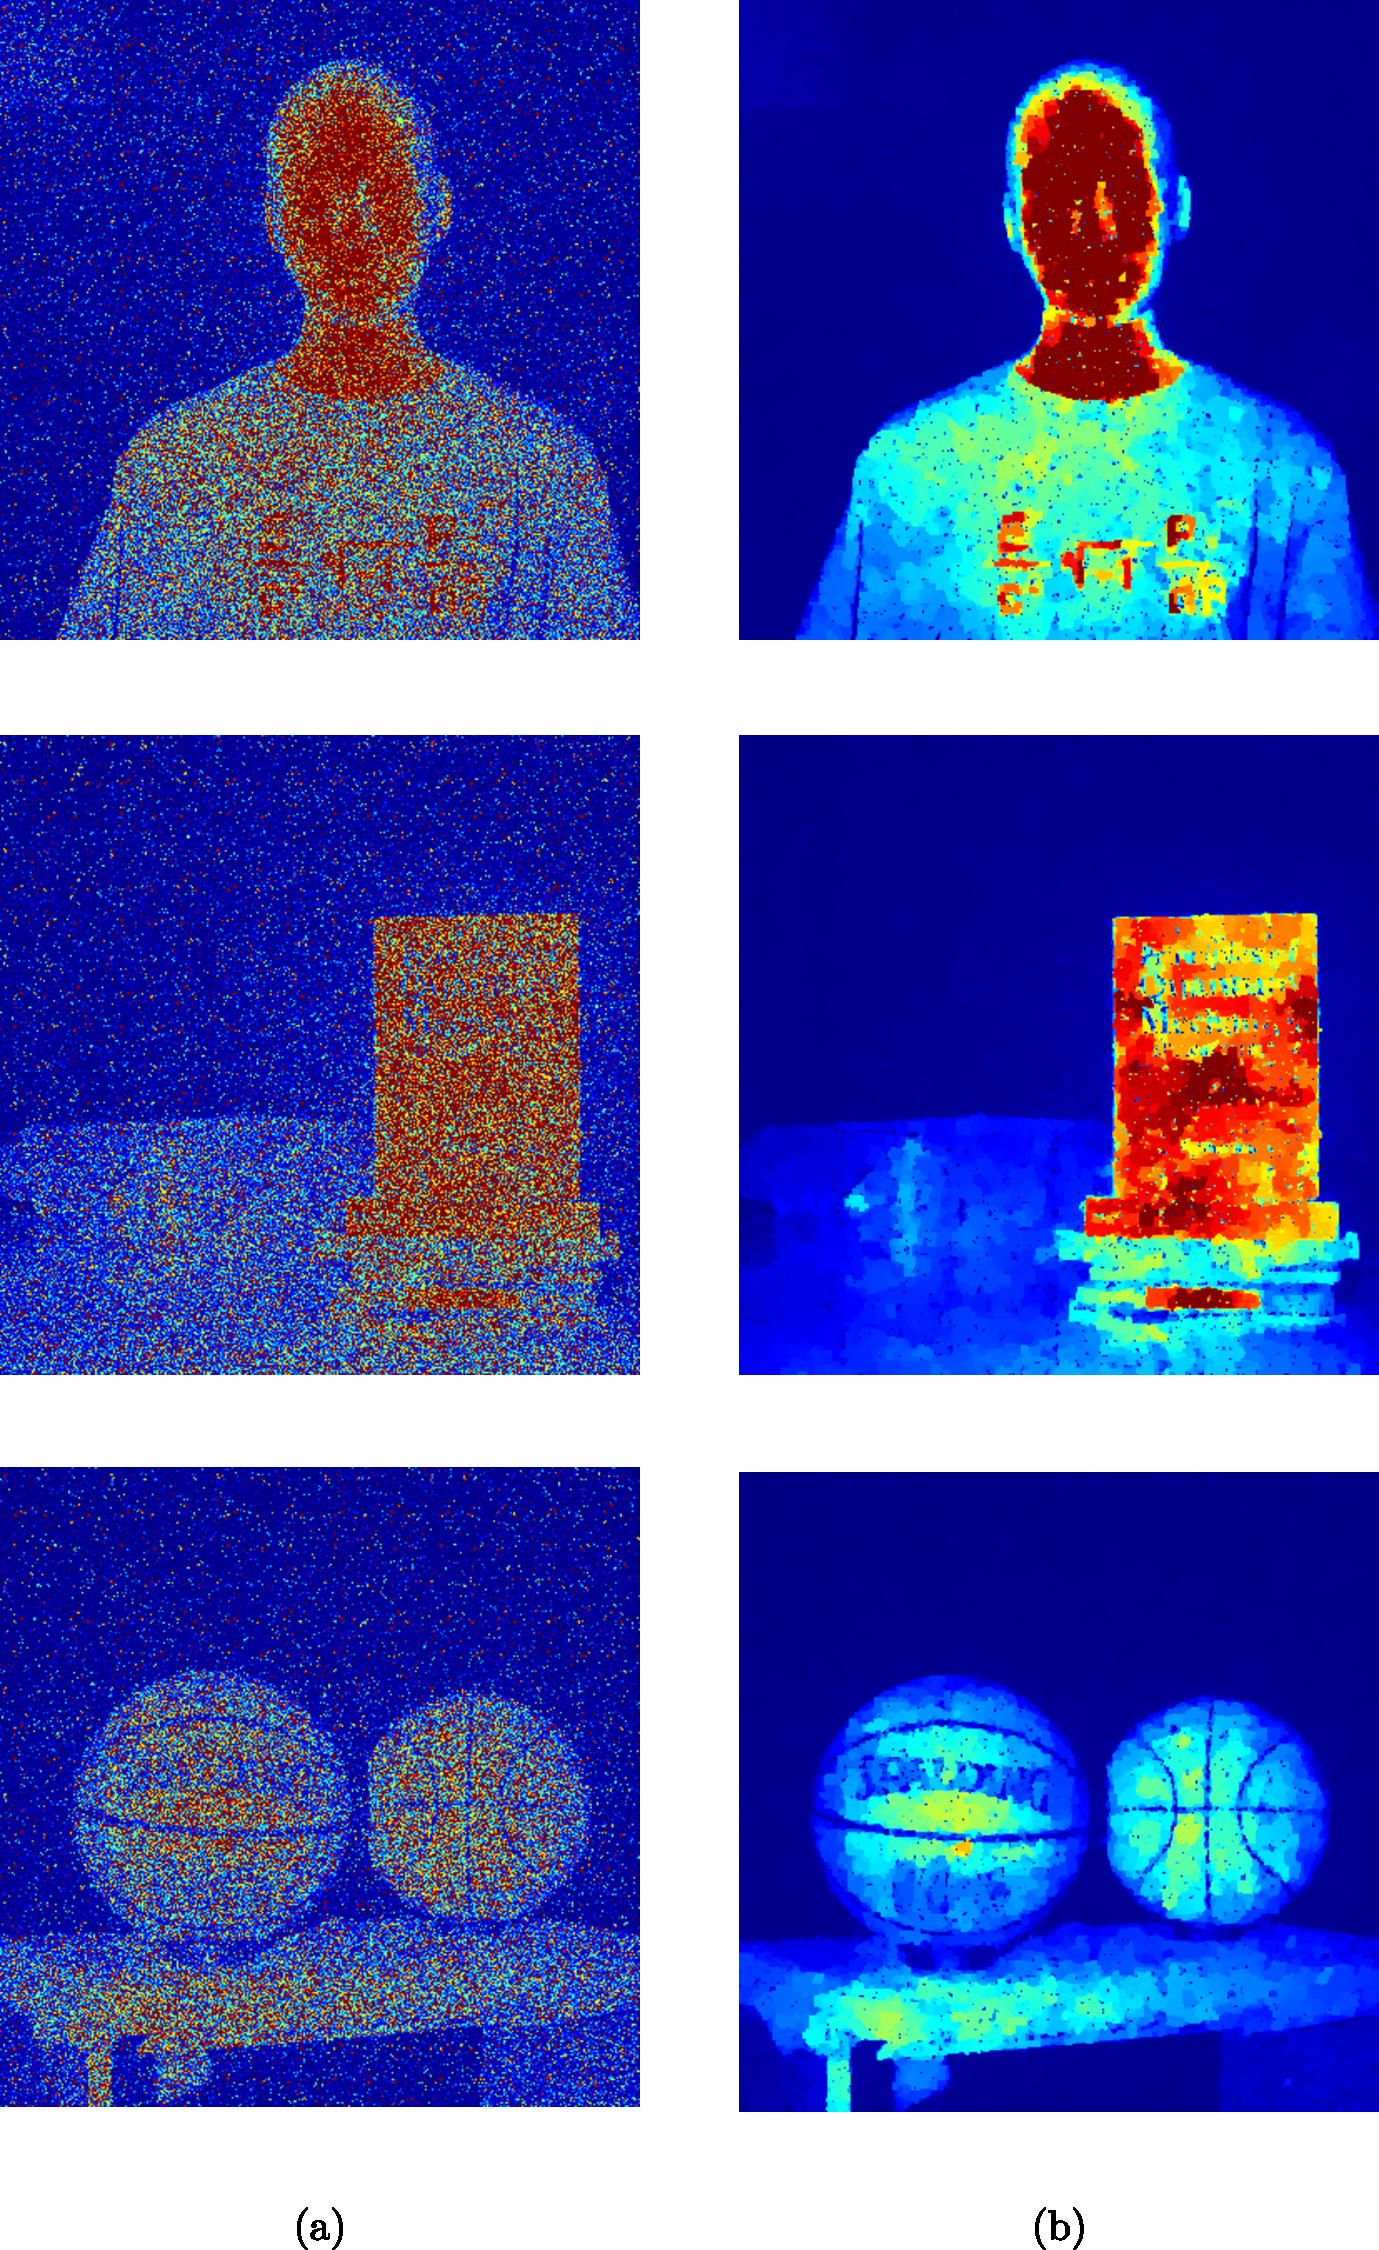
\includegraphics[width=11cm]{figure-first-spad-first-i.pdf}}
\caption{First-photon reflectivity imaging of three scenes simulated using the SPAD array, in which only the first arrival at each pixel is employed regardless of subsequent arrivals within a fixed dwell time. (a) Pixel-wise ML estimate of the reflectivity and (b) the same data after processing using our first-photon imaging technique described in the previous section. Depth results are not generated because $s(\cdot)$ is nearly a delta function for the laser pulse width and time bin size used.}
\label{figure:first-spad-first-i}
\end{figure}

Although the reflectivity images demonstrated some level of improvement using computational reconstruction, we found that with our imaging parameters and object size, it was difficult to obtain significant improvements in the depth maps. As shown in Figure \ref{figure:first-spad-mannequin-d}, at a dwell time of 25 frames, there was simply not enough data in the image to obtain a depth map. This is because although pixels with no data provide us with valid information about reflectivity (the lack of arrivals at a pixel during a particular dwell time period can be interpreted as reflectivity information using Poisson statistics), the no-data pixels provide no depth information, causing the depth reconstruction stage to suffer.

On the other hand, when the dwell time was increased to $\sim$400 frames or more, we obtained enough counts to form a higher-quality depth map, but computational reconstruction failed to extract significant features unseen in the pixel-wise ML estimate. We attribute this to a mismatch between the SPAD specifications, laser pulse width, and the imaging target. In contrast to our first-photon imaging experiment in which the time bin size of the HydraHarp is much shorter than the duration of the laser pulse, the time bin duration of the SPAD array was actually much longer than the laser pulse. This means that $s(\cdot)$ is effectively only 1-2 time bins in size (in contrast to $\sim$28 bins for our raster-scanning experiment) and an object with small variations in the axial direction becomes nearly obliterated by the quantization error of the bin size. We expect that the particular SPAD array we used would lend itself to more fruitful depth reconstruction experiments if we were to use a laser pulse much longer than the time bin duration, e.g., at least 1-2 ns, and a large object with depth features at least 1/10 of the pulse width. Under these conditions we expect to see a stronger difference between the depth-resolving capabilities of traditional imaging and our sparsity-based reconstruction technique.

\begin{figure}[h!]
\centerline{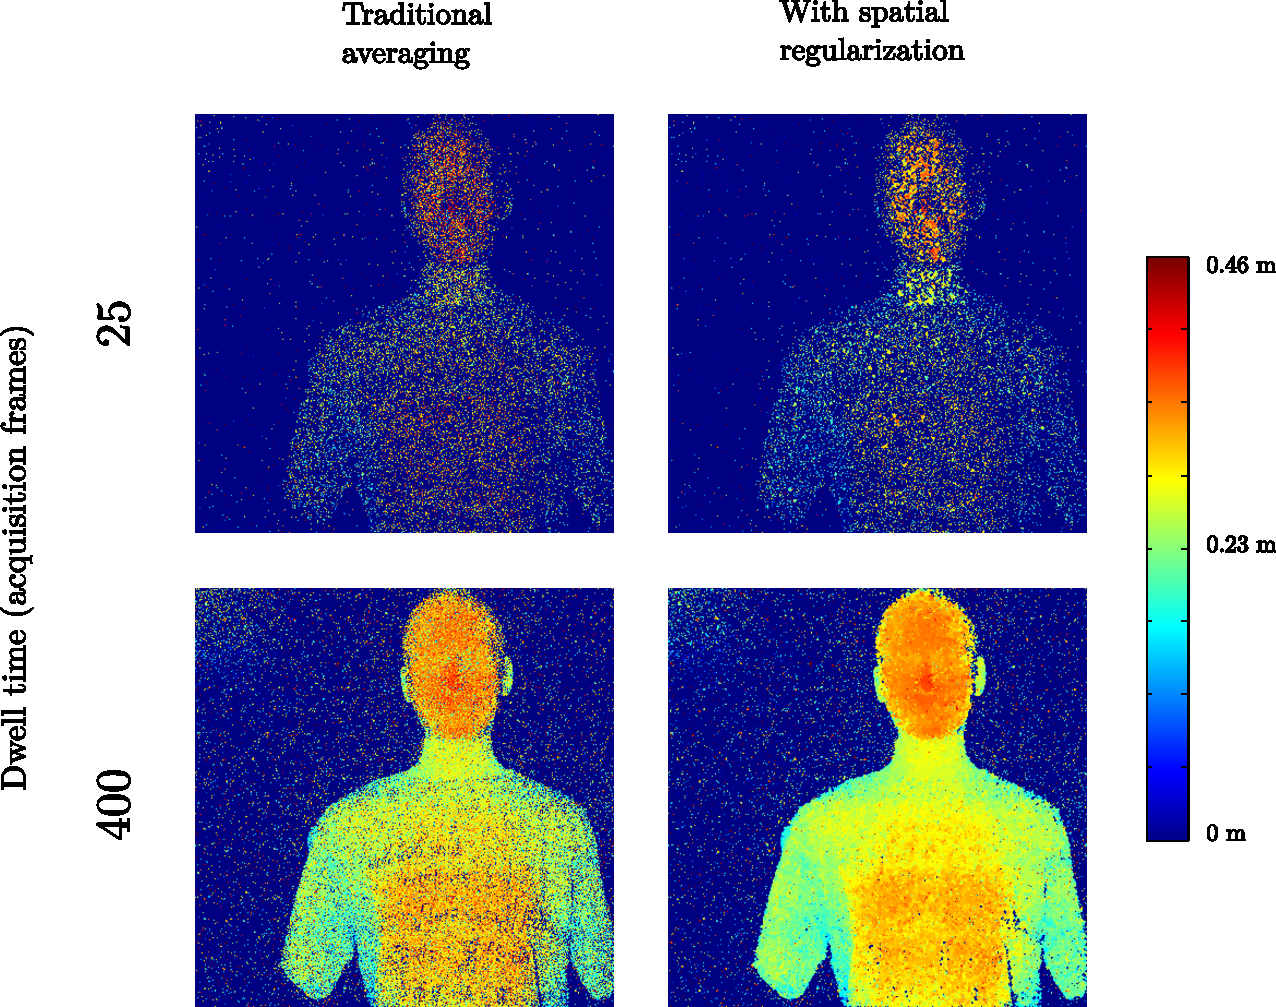
\includegraphics[width=15cm]{figure-first-spad-mannequin-d.pdf}}
\caption{SPAD array imaging results for 360$\times$360-pixel depth maps of a mannequin comparing traditional averaging with spatial regularization. Dwell times are in time units of acquisition frames (65 $\mu$s). Pixels with no data are represented as depth values of $0$.}
\label{figure:first-spad-mannequin-d}
\end{figure}

\section{Conclusions}

In this chapter we explored imagers that use extremely low photon fluxes to capture three-dimensional structure and reflectivity information about an object. Such imagers have wide commercial applications including in medicine, military, and mobile applications. Current imaging technologies, including LIDAR, typically acquire and histogram hundreds of photon arrivals per pixel in order to accumulate a clean image.

These traditional imagers treat each pixel as an independent statistical process and ignore the spatial correlations between pixels that arise from piecewise smoothly-varying structures in real-world scenes. We present a novel imaging paradigm that is designed to take advantage of this property, captured well by sparsity in a wavelet transform basis, and computationally reconstructs the most likely image given a much smaller set of data.

We experimentally demonstrated first-photon imaging, an active imaging method by which we only acquire the first photon arrival at every pixel before moving on to the next pixel. We demonstrated a level of resolution in both reflectivity and depth similar to images obtained using hundreds of photon arrivals, effectively improving the photon efficiency of our imager by a factor of $\sim$100, which is crucial for remote sensing at longer distances with power-limited transmitters. It also enables us to reduce the active illumination power, which is of value in imaging sensitive biological samples, fluorescence-lifetime imaging, mobile devices, robotics, and military applications.

We also adapted our first-photon imaging technique to the case of fixed, deterministic dwell times in order to take advantage of recent developments in SPAD arrays with time-resolving photon detectors at every pixel, that enable an entire image to be acquired in parallel without raster scanning. We established a research collaboration with the Zappa group at the Politecnico di Milano, which has developed a prototype SPAD array. Preliminary results showed improvements in reflectivity estimation, but we found that due to a mismatch between our laser pulse, SPAD array time resolution, and object size, we were not able to perform a thorough test of the method's capabilities.

Future research in single-photon imaging may improve upon our methods in background light suppression, intelligent range gating, advances in detector technologies, as well as applying computational reconstruction to other forms of imaging or sensing in which sparsity and spatial structure can be exploited.


